% Team 02 - Mid-Term Presentation: Anomaly Detection and Causal Analysis Pipeline
% Professional German University Style LaTeX Beamer Presentation

\documentclass[aspectratio=169, 11pt]{beamer}

% ============================================================================
% THEME CONFIGURATION - German University Style
% ============================================================================
\usetheme{Madrid}
\usecolortheme{whale}
\useoutertheme[subsection=false]{miniframes}

% Custom colors inspired by German universities (e.g., TU/LMU style)
\definecolor{uniblue}{RGB}{0, 51, 102}
\definecolor{unigray}{RGB}{85, 85, 85}
\definecolor{lightgray}{RGB}{240, 240, 240}
\definecolor{accentred}{RGB}{153, 0, 0}

% Apply custom colors
\setbeamercolor{structure}{fg=uniblue}
\setbeamercolor{frametitle}{bg=uniblue, fg=white}
\setbeamercolor{title}{bg=uniblue, fg=white}
\setbeamercolor{block title}{bg=uniblue, fg=white}
\setbeamercolor{block body}{bg=lightgray, fg=black}
\setbeamercolor{item}{fg=uniblue}
\setbeamercolor{subitem}{fg=unigray}
\setbeamercolor{footline}{fg=unigray}
\setbeamercolor{section in head/foot}{fg=white, bg=uniblue}
\setbeamercolor{mini frame}{fg=white, bg=uniblue}
\setbeamerfont{section in head/foot}{size=\scriptsize}
\setbeamerfont{section title}{size=\LARGE, series=\bfseries}

% Remove navigation symbols
\setbeamertemplate{navigation symbols}{}

% Custom footline
\setbeamertemplate{footline}{
  \leavevmode%
  \hbox{%
    \begin{beamercolorbox}[wd=.333333\paperwidth,ht=2.25ex,dp=1ex,center]{author in head/foot}%
      \usebeamerfont{author in head/foot}\insertshortauthor
    \end{beamercolorbox}%
    \begin{beamercolorbox}[wd=.333333\paperwidth,ht=2.25ex,dp=1ex,center]{title in head/foot}%
      \usebeamerfont{title in head/foot}\insertshorttitle
    \end{beamercolorbox}%
    \begin{beamercolorbox}[wd=.333333\paperwidth,ht=2.25ex,dp=1ex,right]{date in head/foot}%
      \usebeamerfont{date in head/foot}\insertshortdate{}\hspace*{2em}
      \insertframenumber{} / \inserttotalframenumber\hspace*{2ex}
    \end{beamercolorbox}}%
  \vskip0pt%
}

% ============================================================================
% PACKAGES
% ============================================================================
\usepackage[utf8]{inputenc}
\usepackage[T1]{fontenc}
\usepackage{lmodern}
\usepackage{amsmath, amssymb}
\usepackage{booktabs}
\usepackage{graphicx}
\usepackage{tikz}
\usepackage{xcolor}
\usepackage{array}
\usepackage{multirow}
\usepackage{hyperref}
\usepackage{listings}
\usetikzlibrary{arrows.meta,positioning,shapes.geometric,shadows}

% Table column types
\newcolumntype{L}[1]{>{\raggedright\arraybackslash}p{#1}}
\newcolumntype{C}[1]{>{\centering\arraybackslash}p{#1}}

% ============================================================================
% TITLE PAGE INFORMATION
% ============================================================================
\title[OMN]{OMN}
% \subtitle{Mid-Term Presentation -- AI Algorithms}
\author[Team 04 Final Presentation]{Team 04 Final Presentation}
\institute[Universität Bremen]{Robot Programing with ROS\\Summer Semester 2026}
\date{Jun 03, 2026}

% Keep a compact label in the top navigation and the full title on dividers.
\newcommand{\fullsectiontitle}{}
\newcommand{\presentationsection}[2][]{%
  \gdef\fullsectiontitle{#2}%
  \section[#1]{#2}%
}

% Dedicated title slide for each section, with the navigation bar visible.
\AtBeginSection[]{
  \begin{frame}
    \centering
    \vfill
    
\begin{tikzpicture}
      \node[
        fill=uniblue,
        text=white,
        rounded corners=8pt,
        drop shadow={shadow xshift=1.5mm, shadow yshift=-1.5mm, opacity=0.45},
        minimum width=0.88\paperwidth,
        minimum height=1.8cm,
        inner xsep=8mm,
        align=center
      ] {\usebeamerfont{section title}\fullsectiontitle};
    \end{tikzpicture}
    \vfill
  \end{frame}
}

% ============================================================================
% DOCUMENT
% ============================================================================
\begin{document}

% Title Slide
\begin{frame}[plain]
  \titlepage
\end{frame}

% Table of Contents
\begin{frame}{Outline}
  \tableofcontents
\end{frame}

% ============================================================================
% BEGIN CONTENT IMPORTED FROM omn.tex
\presentationsection[Overview]{Overview}


\begin{frame}{Overview}
    \begin{figure}
        \centering
        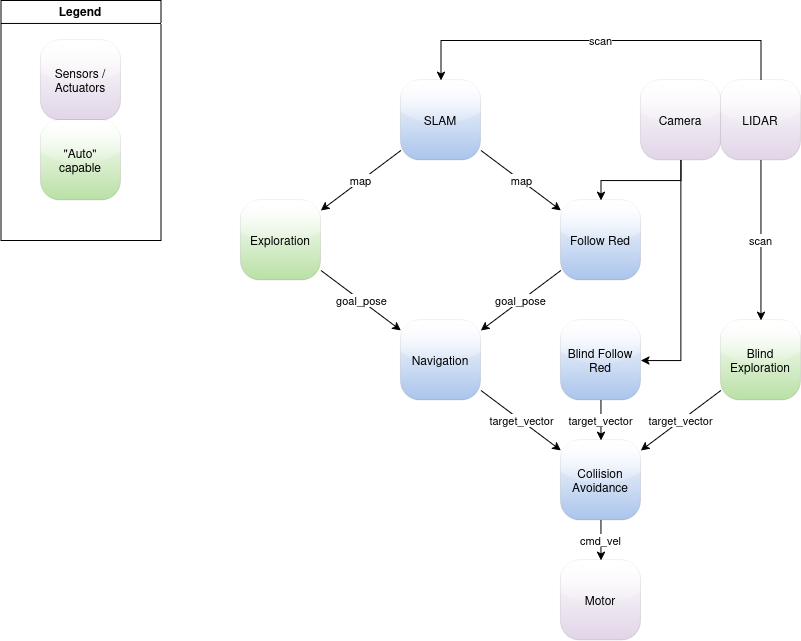
\includegraphics[width=0.5\linewidth]{img/overview.drawio.png}
    \end{figure}
\end{frame}


% ============================================================================
% EXPLORATION
% ============================================================================
\presentationsection[Exploration]{Exploration}


\begin{frame}{Blind Exploration}
    \begin{itemize}
        \item No map given
    \end{itemize}
    
    To complete the main goal \textit{"Just keep moving!"} we do this:
    
    \begin{enumerate}
        \item Apply random drift
        \item Drive forward
        \item Wall detected?
        \begin{enumerate}
            \item Yes: apply force to the side of the wall
        \end{enumerate}
        \item Haven't moved for a while?
        \begin{enumerate}
            \item Yes: apply randomized rotation
        \end{enumerate}
    \end{enumerate}
\end{frame}

\begin{frame}{Blind Exploration}
    \begin{figure}
        \centering
        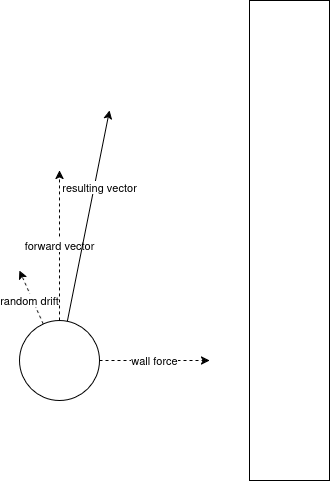
\includegraphics[width=0.38\linewidth]{img/blind_exploration.drawio.png}
    \end{figure}
\end{frame}

\begin{frame}{Blind Exploration - Why the drift?}
    \begin{figure}
        \centering
        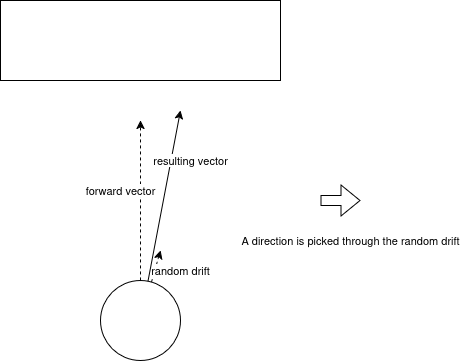
\includegraphics[width=0.6\linewidth]{img/random_drift.drawio.png}
    \end{figure}
\end{frame}

\begin{frame}{Exploration}
    \begin{itemize}
        \item Sufficient exploration has taken place
        \item Map given
    \end{itemize}
    
    We now know where we are and where we've been, the goal changes to \textit{"Explore the unknown!"}:

    \begin{enumerate}
        \item Flood fill the map from our current position
        \item Create a frontier map
        \item Select the closes frontier position (we haven't visited yet)
        \item Send desired location to \lstinline{/goal_pose}
        \item Mark position as visited
    \end{enumerate}
\end{frame}

\begin{frame}{Exploration}
    \begin{figure}
        \centering
        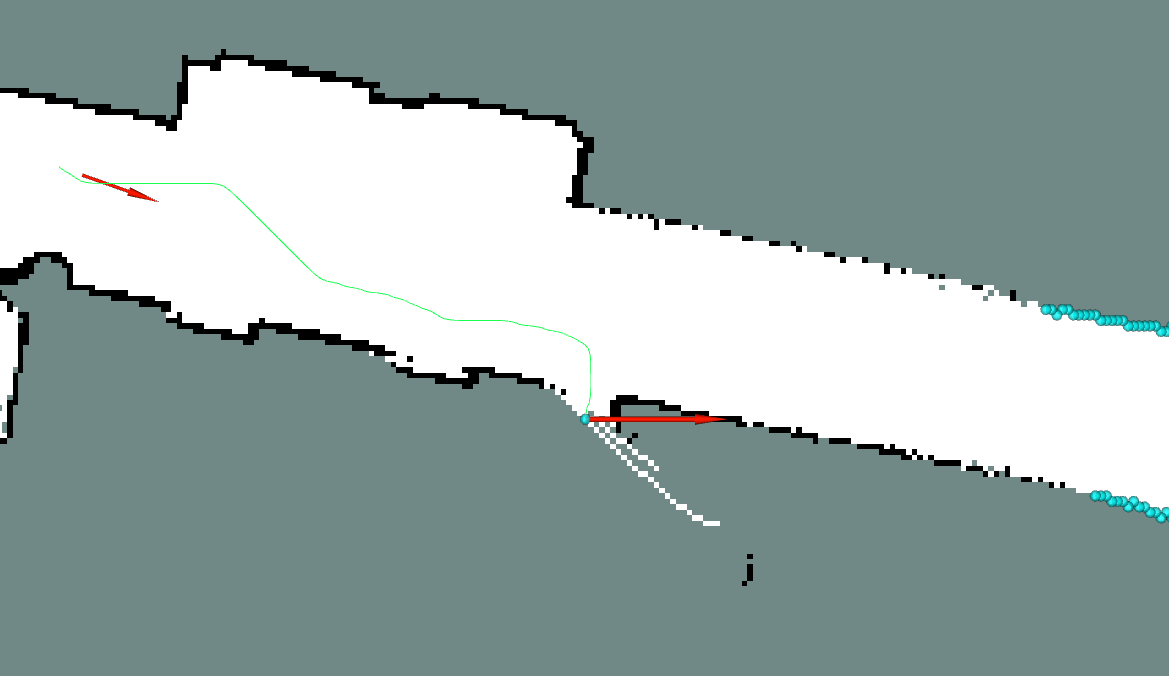
\includegraphics[width=\linewidth]{img/exploration.png}
    \end{figure}
\end{frame}


% ============================================================================
% COLLISION AVOIDANCE
% ============================================================================
\presentationsection[Collision Avoidance]{Collision Avoidance}


\begin{frame}{Collision Avoidance}
    \begin{itemize}
        \item Has to be active if the robot wants to move
        \item Receives an \lstinline{/target_vector} with a linear and angular velocity
        \item Ensures...
        \begin{itemize}
            \item that the velocities are within safe bounds
            \item that the movement direction does not point into obstacles
        \end{itemize}
        \item Converts \lstinline{/target_vector} to \lstinline{/cmd_vel} and sends it off to motor
    \end{itemize}
\end{frame}

\begin{frame}{Collision Avoidance}
    \begin{figure}
        \centering
        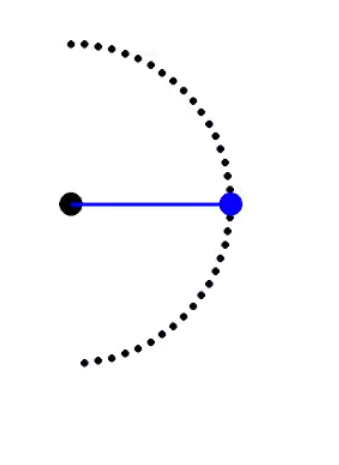
\includegraphics[width=0.4\linewidth]{img/coll_av_idle.png}
    \end{figure}
\end{frame}

\begin{frame}{Collision Avoidance}
    \begin{figure}
        \centering
        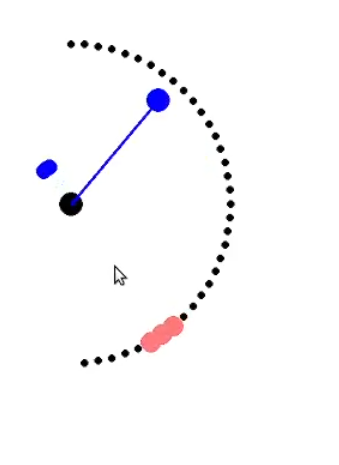
\includegraphics[width=0.4\linewidth]{img/coll_av.png}
    \end{figure}
\end{frame}

% ============================================================================
\presentationsection[Navigation]{Navigation}
% ============================================================================

\begin{frame}{Navigation Steps:}
  \small
  \begin{columns}[T]
    \begin{column}{0.48\textwidth}
      \begin{block}{Planning}
        \begin{enumerate}
          \item \texttt{timer\_callback()} waits until a map, pose, and goal are available.
          \item Robot and goal positions are converted from metres to map-grid cells.
          \item A* plans a path using horizontal, vertical, and diagonal moves.
          \item Obstacles are inflated to maintain clearance, and the grid path is smoothed to reduce zig-zag motion.
        \end{enumerate}
      \end{block}
    \end{column}

    \begin{column}{0.48\textwidth}
      \begin{block}{Path Following}
        \begin{enumerate}
          \setcounter{enumi}{4}
          \item Every $0.2\,\mathrm{s}$, a waypoint approximately $0.4\,\mathrm{m}$ ahead is selected.
          \item A \texttt{TargetVector} pointing toward the waypoint is published.
          \item When the goal is within $0.4\,\mathrm{m}$, the robot is stopped and \texttt{goal\_succeeded} is reported.
        \end{enumerate}
      \end{block}
    \end{column}
  \end{columns}
\end{frame}

\begin{frame}{A* Path Planning}
  \begin{columns}[T]
    \begin{column}{0.55\textwidth}
      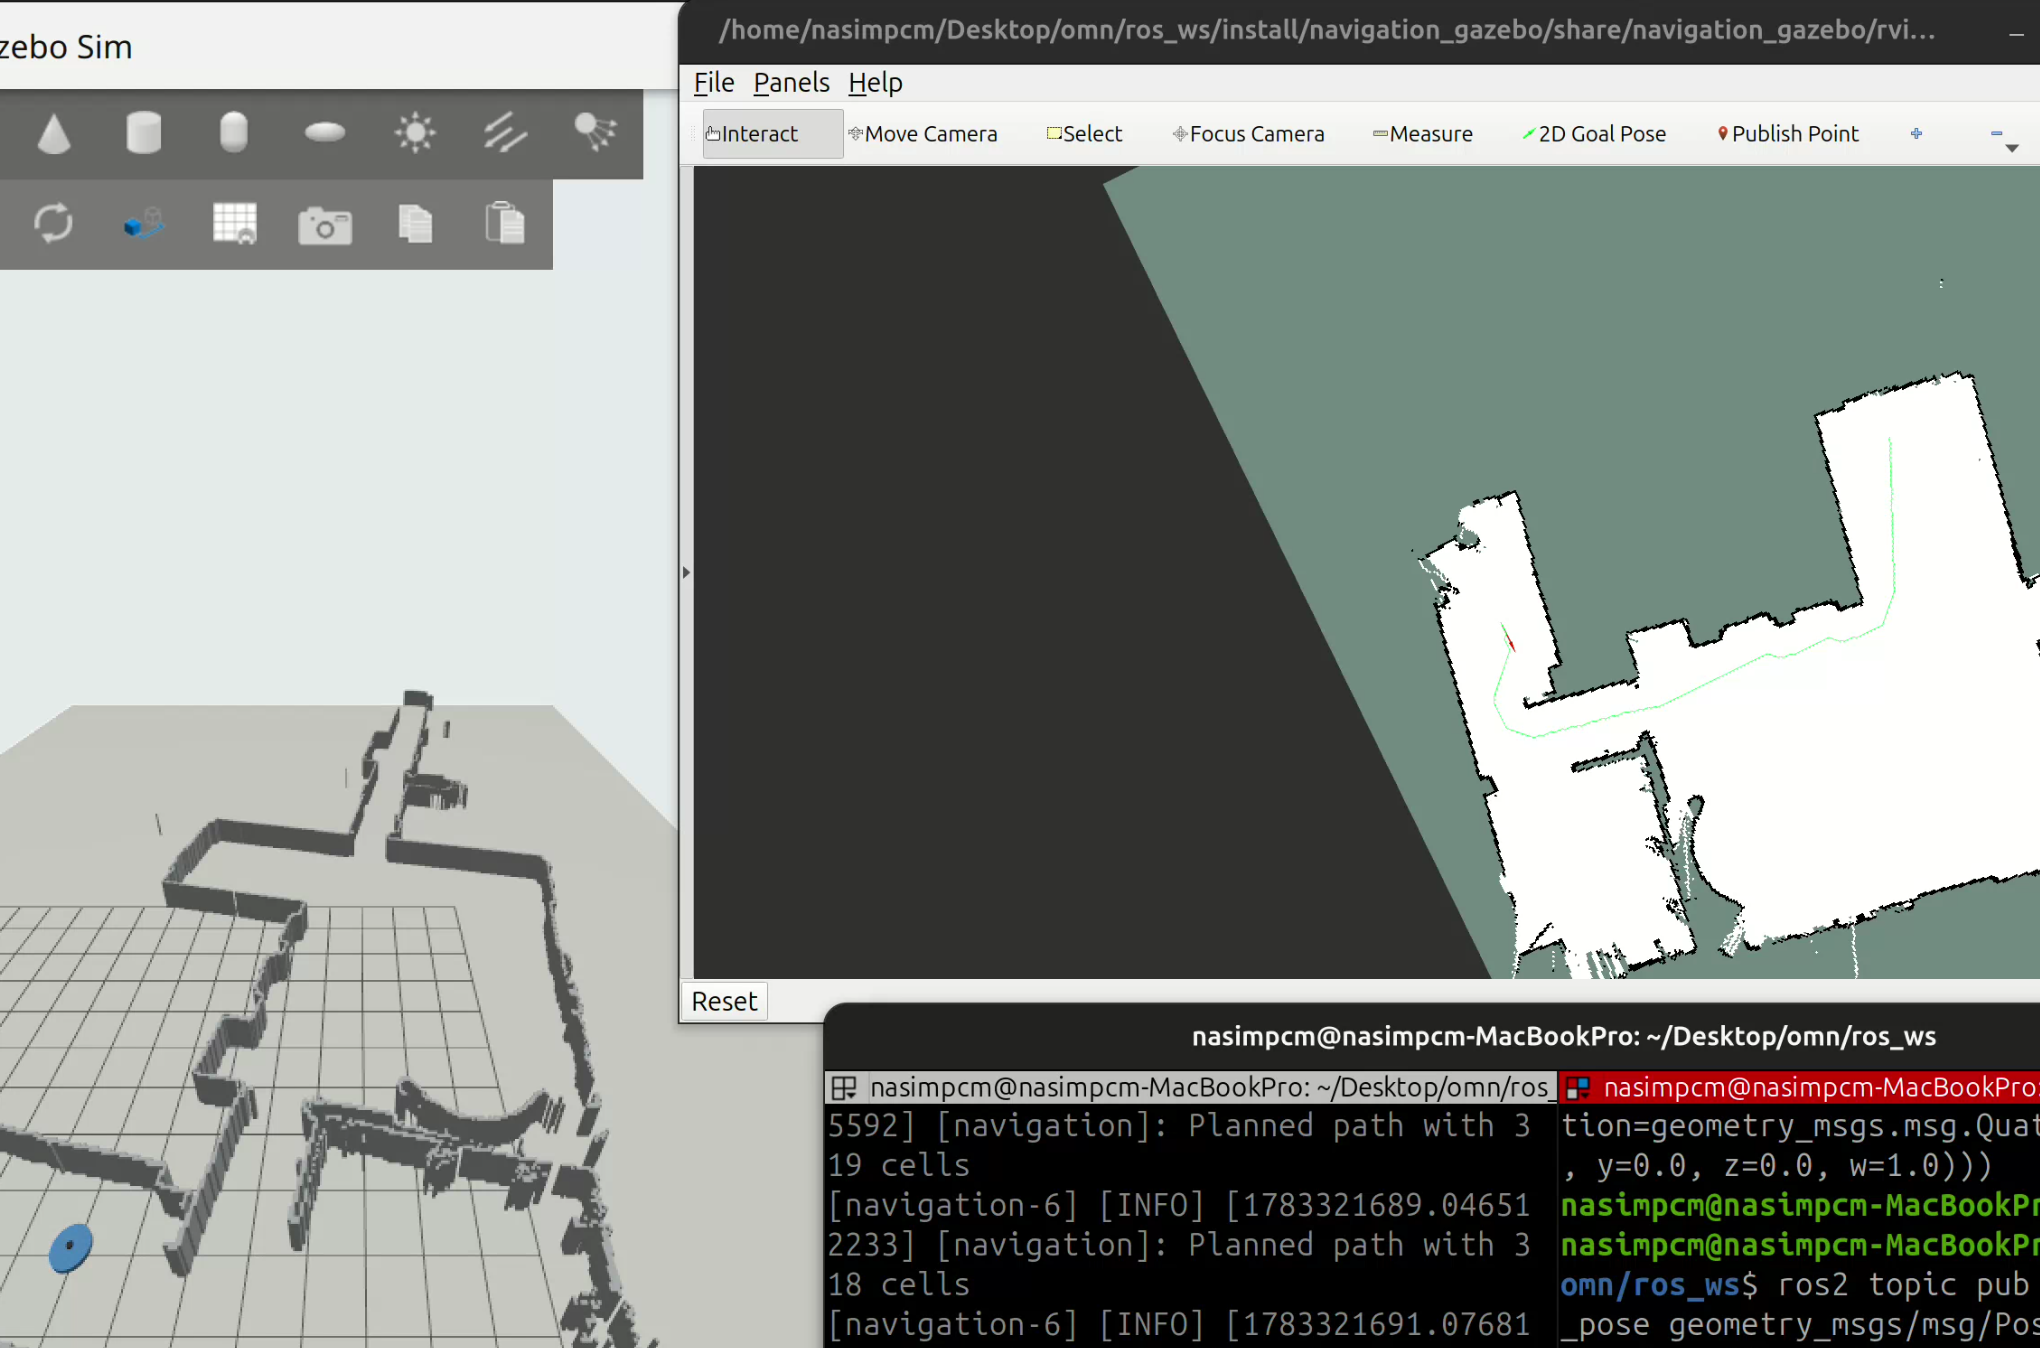
\includegraphics[width=\textwidth,height=0.68\textheight,keepaspectratio]{img/nav.png}
    \end{column}

    \begin{column}{0.41\textwidth}
      \begin{block}{Evaluation Function}
        \begin{equation*}
          f(n)=g(n)+h(n)
        \end{equation*}
        \footnotesize
        $g(n)$ is the path cost from the start and $h(n)$ estimates the remaining cost to the goal.
      \end{block}

      \begin{itemize}
        \item Eight-connected grid search
        \item Straight-move cost: $1$
        \item Diagonal-move cost: $\sqrt{2}$
      \end{itemize}
    \end{column}
  \end{columns}
\end{frame}

\begin{frame}{A* Implementation}
  \small
  \begin{columns}[T]
    \begin{column}{0.48\textwidth}
      \begin{enumerate}
        \item \textbf{Initialize:} add the start cell to the open-set priority queue, set $g(\text{start})=0$, and initialize \texttt{came\_from}, \texttt{g\_score}, and the closed set.
        \item \textbf{Select:} remove the cell with the smallest estimated total cost $f(n)$.
        \item \textbf{Check the goal:} if selected, reconstruct the path from the stored parent cells.
        \item \textbf{Mark explored:} skip cells already processed; otherwise add the cell to the closed set.
      \end{enumerate}
    \end{column}

    \begin{column}{0.48\textwidth}
      \begin{enumerate}
        \setcounter{enumi}{4}
        \item \textbf{Generate neighbors:} consider all eight adjacent cells using straight and diagonal move costs.
        \item \textbf{Apply obstacle costs:} reject blocked or invalid cells and penalize inflated cells near obstacles.
        \item \textbf{Update better paths:} if a lower cost is found, update the neighbor's parent and scores, then add it to the open set.
        \item \textbf{Finish:} return the reconstructed path, or report \texttt{no\_path} if the open set becomes empty.
      \end{enumerate}
    \end{column}
  \end{columns}
\end{frame}

\begin{frame}{Next Waypoint Selection}
  \small
  \begin{columns}[T]
    \begin{column}{0.52\textwidth}
      \begin{block}{1. Locate the Robot on the Path}
        Project the robot onto every remaining path segment and select the closest point $P$.
      \end{block}

      \begin{block}{2. Look Ahead Along the Path}
        Starting at $P$, measure $0.40\,\mathrm{m}$ along the path to obtain waypoint $W$. If the distance crosses a corner, continue on the next segment.
      \end{block}

      \begin{itemize}
        \item \texttt{path\_progress} prevents the selected position from jumping backward when the path passes close to itself.
        \item If less than $0.40\,\mathrm{m}$ remains, return the final goal point.
      \end{itemize}
    \end{column}

    \begin{column}{0.44\textwidth}
      \centering
      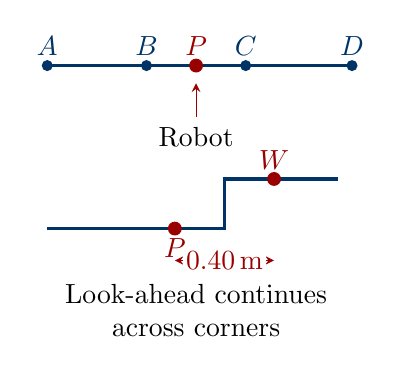
\begin{tikzpicture}[x=0.9cm,y=0.9cm,>=stealth]
        \draw[very thick,uniblue] (0,3.8) -- (1.4,3.8) -- (2.8,3.8) -- (4.3,3.8);
        \fill[uniblue] (0,3.8) circle (2pt) node[above] {$A$};
        \fill[uniblue] (1.4,3.8) circle (2pt) node[above] {$B$};
        \fill[uniblue] (2.8,3.8) circle (2pt) node[above] {$C$};
        \fill[uniblue] (4.3,3.8) circle (2pt) node[above] {$D$};
        \fill[accentred] (2.1,3.8) circle (2.5pt) node[above] {$P$};
        \node (robot) at (2.1,2.8) {Robot};
        \draw[->,accentred] (robot) -- (2.1,3.55);

        \draw[very thick,uniblue] (0,1.5) -- (1.4,1.5) -- (2.5,1.5) -- (2.5,2.2) -- (4.1,2.2);
        \fill[accentred] (1.8,1.5) circle (2.5pt) node[below] {$P$};
        \fill[accentred] (3.2,2.2) circle (2.5pt) node[above] {$W$};
        \draw[<->,accentred] (1.8,1.05) -- node[fill=white,inner sep=1pt] {$0.40\,\mathrm{m}$} (3.2,1.05);
        \node[align=center] at (2.1,0.35) {Look-ahead continues\\across corners};
      \end{tikzpicture}
    \end{column}
  \end{columns}
\end{frame}

% ============================================================================
% FOLLOW RED
% ============================================================================
\presentationsection[Follow Red]{Follow Red}
\begin{frame}{Goal in 3 Steps}
    \begin{enumerate}
        \item Detect a red cube via OpenCV
        \item Estimate its distance/angle or global map position 
        \item Publish targets in a ROS 2 system
    \end{enumerate}

    \vspace{0.3cm}
    \begin{itemize}
        \item \textbf{Node Type:} ROS 2 Lifecycle Node
        \item \textbf{Input:} OpenCV camera stream
        \item \textbf{Processing:} HSV masking, exponential smoothing, median filtering
        \item \textbf{Output:} Polar coordinates (\texttt{TargetVector}) or global map poses (\texttt{PoseStamped})
    \end{itemize}
\end{frame}

\begin{frame}{Given Hardware and Calibration}
    \begin{table}[]
        \centering
        \begin{tabular}{c|c}
             Type & Webcam \\
             Frame & 640x480 \\
             FOV & 60 \\
             Calibrated Distance & 1 Meter \\
             Calibrated Pixels & 9750
        \end{tabular}
    \end{table}
\end{frame}

\begin{frame}{Dual Target Publishing Modes}
    Controlled by the runtime parameter \texttt{send\_polar}:

    \vspace{0.4cm}
    \begin{columns}[t]
        \begin{column}{0.48\textwidth}
            \begin{block}{Polar Mode (\texttt{send\_polar = True})}
                \begin{itemize}
                    \item Publishes \texttt{TargetVector} to \texttt{/target\_vector}.
                    \item Direct values for \texttt{linear} (distance) and \texttt{angular} (bearing angle).
                \end{itemize}
            \end{block}
        \end{column}
        
        \begin{column}{0.48\textwidth}
            \begin{block}{Global Pose Mode (\texttt{send\_polar = False})}
                \begin{itemize}
                    \item Uses \texttt{tf2\_ros} for transform lookups (\texttt{map} $\rightarrow$ \texttt{base\_footprint}).
                    \item Transforms camera relative coordinates into global map coordinates.
                    \item Publishes \texttt{PoseStamped} to \texttt{/goal\_pose}.
                \end{itemize}
            \end{block}
        \end{column}
    \end{columns}
\end{frame}

\begin{frame}{Image Processing \& Filter Pipeline}
    \begin{enumerate}
        \item \textbf{Filter Size:}
            \begin{itemize}
                \item Accept only a sum over 500px as possible cube.
            \end{itemize}
        \item \textbf{Area Change Rate Filter (Jump Filter):}
            \begin{itemize}
                \item Ignores frames with sudden, extreme area size spikes ($\frac{A_{\text{new}}}{A_{\text{old}}} \notin [\text{min}, \text{max}]$).
                \item Prevents position jumps caused by brief reflections or partial occlusions.
            \end{itemize}
        \item \textbf{HSV Masking:}
            \begin{itemize}
                \item Dual range masking for red hue due to HSV wrap-around ($0^\circ{-}5^\circ$ and $174^\circ{-}179^\circ$).
            \end{itemize}
        \item \textbf{Low-Pass Filter (Exponential Smoothing):}
            \begin{itemize}
                \item Noise reduction for pixel position ($\alpha_{\text{pos}} = 0.25$) and area ($\alpha_{\text{area}} = 0.20$).
            \end{itemize}
        \item \textbf{Median Ring Buffer:}
            \begin{itemize}
                \item \texttt{deque(maxlen=5)} eliminates sporadic false detections over 5 frames.
            \end{itemize}
        \item \textbf{Distance Estimation:}
            \begin{itemize}
                \item Inverse square-root calculation based on calibrated pixel area:
                $$d = d_0 \cdot \sqrt{\frac{A_0}{A}}$$
            \end{itemize}
    \end{enumerate}
\end{frame}

\begin{frame}{Fault Tolerance}
    \begin{block}{Automatic Camera Reconnect}
        \begin{itemize}
            \item Monitors consecutive read errors
            \item When reaching \texttt{CAMERA\_MAX\_ERRORS} (40 frames $\approx$ 2\,s), the video device is released and re-initialized.
        \end{itemize}
    \end{block}
\end{frame}

% ============================================================================
% MANAGER
% ============================================================================
\presentationsection[Manager]{Manager}


\begin{frame}{Dashboard}
    \begin{figure}
        \centering
        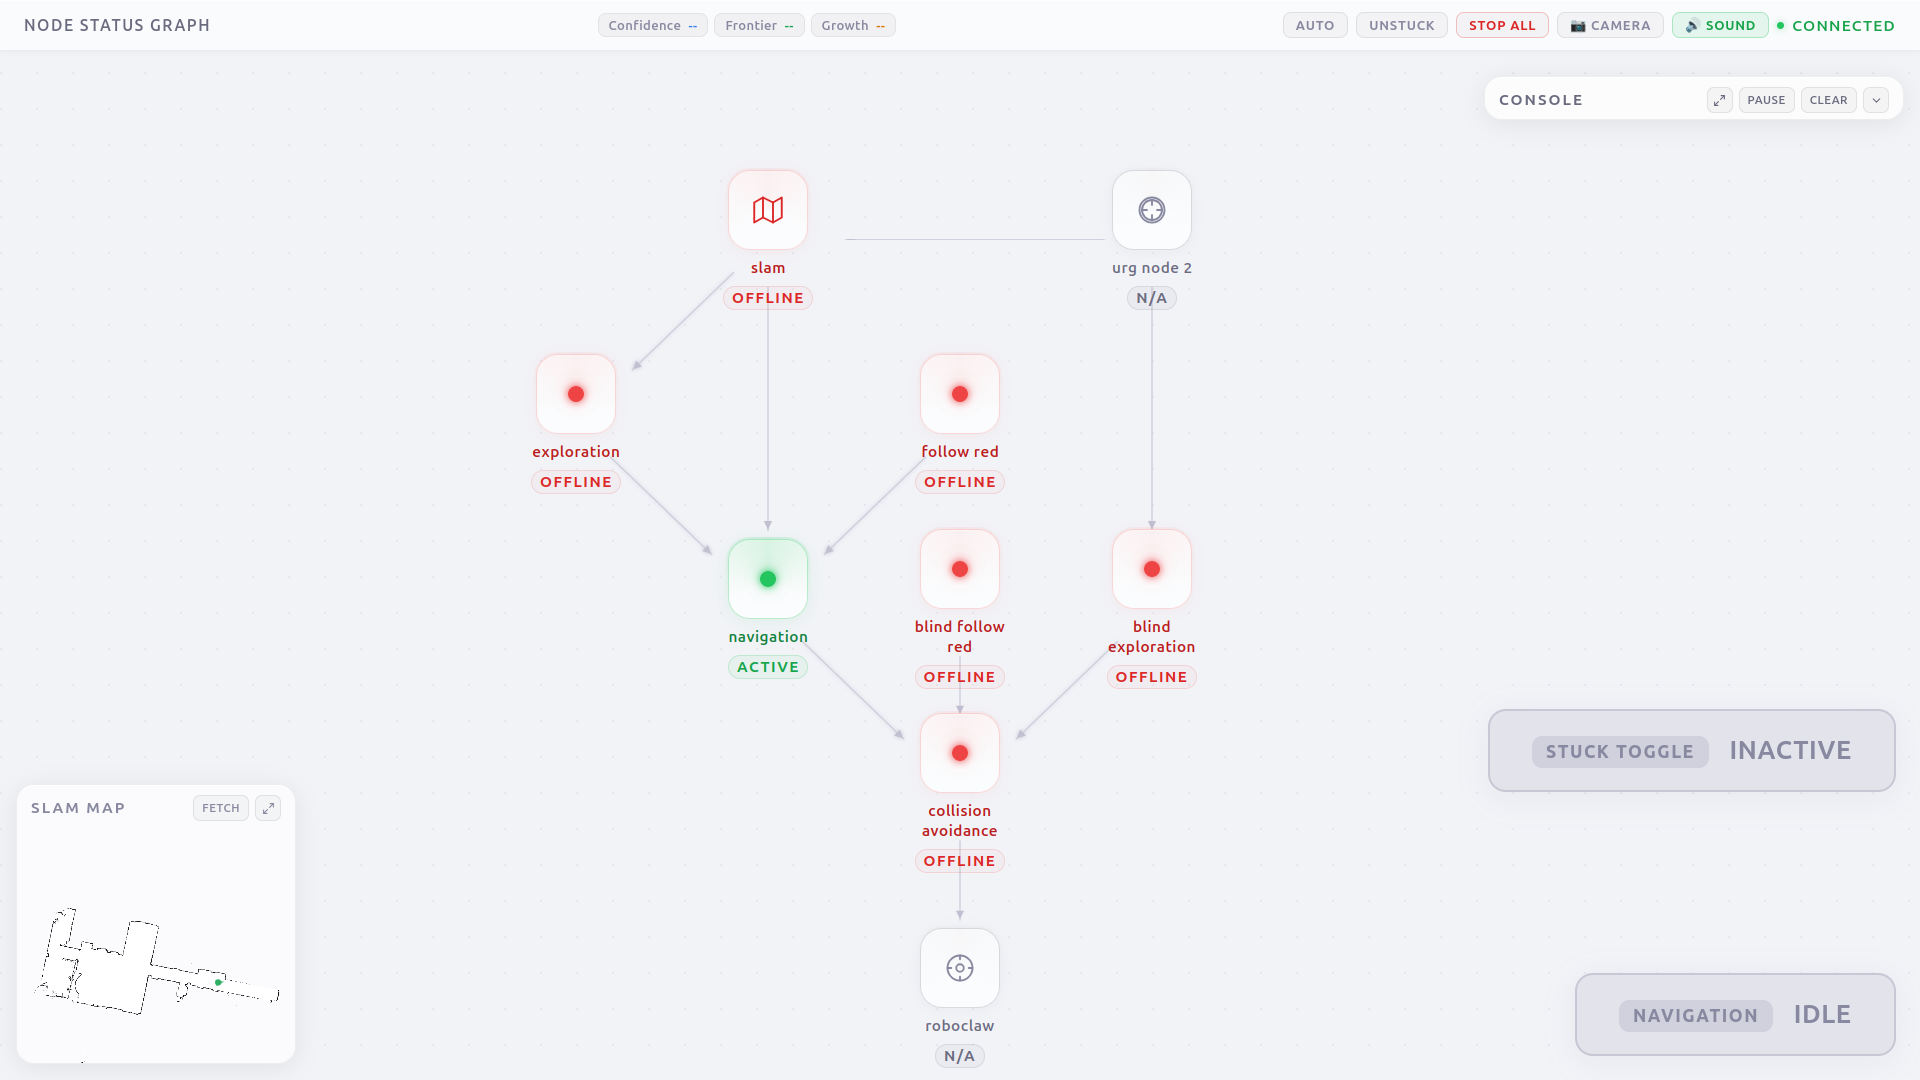
\includegraphics[width=0.7\linewidth]{img/dashboard_1.png}
    \end{figure}
\end{frame}


% ----------------------------------------------------------------------------
% ROBOT MANAGER -- FUNCTIONALITY DEEP DIVE (added slides, native theme style)
% ----------------------------------------------------------------------------

% --- Divider, matches the \AtBeginSection style used elsewhere ---
\begin{frame}
  \vfill
  \centering
  \begin{beamercolorbox}[sep=8pt,center,shadow=true,rounded=true]{title}
    \usebeamerfont{title}Robot Manager -- Functionality Deep Dive\par%
  \end{beamercolorbox}
  \vfill
\end{frame}

% --- 1: Health & Fault Detection ---
\begin{frame}{Health \& Fault Detection} 
  \small
  Every vital system is timed. Silence past a threshold is treated as failure -- automatically.
  \vspace{0.25cm}
  \begin{columns}[T]
    \begin{column}{0.48\textwidth}
      \begin{block}{1 -- LiDAR \texttt{/scan}}
        \footnotesize
        \begin{itemize}
          \item $0\,\mathrm{s}$: healthy
          \item $1.5\,\mathrm{s}$: \textcolor{orange!80!black}{\textbf{WARN}}
          \item $4\,\mathrm{s}$: \textcolor{accentred}{\textbf{DOWN}} -- zero speed forced, task cancelled, state $\rightarrow$ FAULT
        \end{itemize}
      \end{block}
    \end{column}
    \begin{column}{0.48\textwidth}
      \begin{block}{2 -- Localization \texttt{/pose}}
        \footnotesize
        \begin{itemize}
          \item $0\,\mathrm{s}$: healthy
          \item $3\,\mathrm{s}$: \textcolor{orange!80!black}{\textbf{WARN}}
          \item $8\,\mathrm{s}$: \textcolor{accentred}{\textbf{DOWN}} -- same recovery as above
        \end{itemize}
      \end{block}
    \end{column}
  \end{columns}
  \vspace{0.25cm}
  \begin{block}{Why thresholds instead of instant failure?}
    \footnotesize
    A single missed message doesn't mean a sensor is broken -- networks and drivers hiccup. Two thresholds (WARN, then DOWN) give a fair grace window before anything drastic happens, while still guaranteeing a fast, automatic stop once it's truly gone. Healthy again $\rightarrow$ back to INITIALIZING (re-verified).
  \end{block}
\end{frame}

% --- 2: Knowing When Mapping Is Actually Done ---
\begin{frame}{Knowing When Mapping Is Actually Done}
  \small
  Confidence must stay above threshold for a sustained hold time -- a single lucky spike doesn't count.
  \begin{columns}[T]
    \begin{column}{0.52\textwidth}
      \begin{center}
      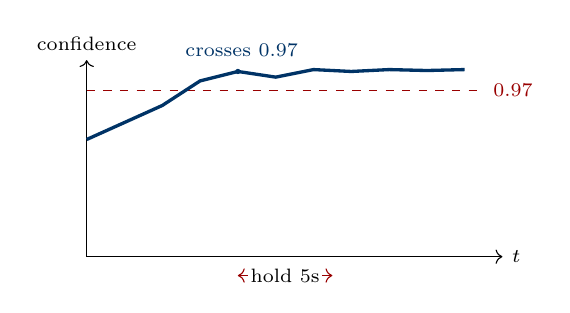
\begin{tikzpicture}[scale=0.48]
        \draw[->] (0,0) -- (11,0) node[right] {\scriptsize $t$};
        \draw[->] (0,0) -- (0,5.2) node[above] {\scriptsize confidence};
        \draw[dashed,accentred] (0,4.4) -- (10.5,4.4);
        \node[right,accentred,font=\scriptsize] at (10.5,4.4) {0.97};
        \draw[very thick,uniblue]
          (0,3.1) -- (1,3.55) -- (2,4.0) -- (3,4.65) -- (4,4.9) -- (5,4.75)
          -- (6,4.95) -- (7,4.9) -- (8,4.95) -- (9,4.925) -- (10,4.95);
        \fill[uniblue] (4,4.9) circle (2pt);
        \node[uniblue,above,font=\scriptsize] at (4.1,5.05) {crosses 0.97};
        \draw[<->,accentred] (4,-0.5) -- (6.5,-0.5);
        \node[fill=white,inner sep=1pt,font=\scriptsize] at (5.25,-0.5) {hold 5s};
      \end{tikzpicture}
      \end{center}
    \end{column}
    \begin{column}{0.44\textwidth}
      \begin{block}{The hold-timer rule}
        \footnotesize
        \begin{enumerate}
          \item Confidence first crosses 0.97 at $\approx 8\,\mathrm{s}$ $\rightarrow$ a hold-timer starts.
          \item It must stay $\geq 0.97$ continuously for 5 more seconds.
          \item Only then is the map declared converged and saved.
        \end{enumerate}
        If it dips below 0.97 even once, the timer resets -- the wait starts fresh.
      \end{block}
    \end{column}
  \end{columns}
\end{frame}

% --- 3: FSM ---
\begin{frame}{How a Finite State Machine (FSM) Runs the Mission}
  \footnotesize
  The robot is always in exactly one state, and a fixed rule table decides every legal transition.
  \begin{center}
  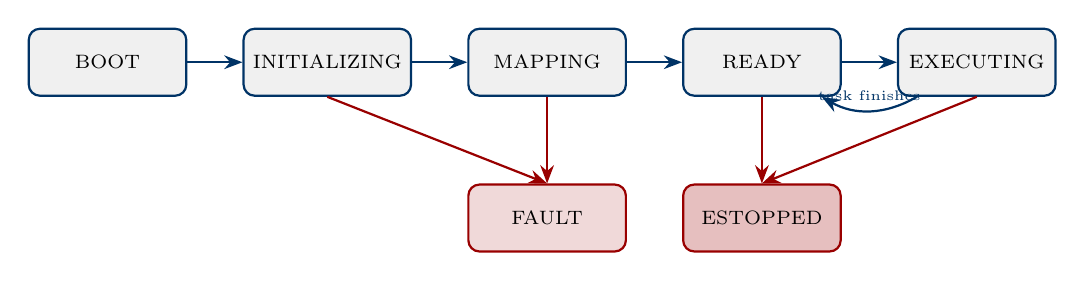
\begin{tikzpicture}[
      state/.style={rectangle,rounded corners,draw=uniblue,thick,fill=lightgray,
        minimum width=2.0cm,minimum height=0.85cm,align=center,font=\scriptsize},
      >=Stealth,thick
    ]
    \node[state] (boot) {BOOT};
    \node[state,right=0.7cm of boot] (init) {INITIALIZING};
    \node[state,right=0.7cm of init] (map) {MAPPING};
    \node[state,right=0.7cm of map] (ready) {READY};
    \node[state,right=0.7cm of ready] (exec) {EXECUTING};
    \node[state,fill=accentred!15,draw=accentred,below=1.1cm of map] (fault) {FAULT};
    \node[state,fill=accentred!25,draw=accentred,below=1.1cm of ready] (estop) {ESTOPPED};

    \draw[->,uniblue] (boot) -- (init);
    \draw[->,uniblue] (init) -- (map);
    \draw[->,uniblue] (map) -- (ready);
    \draw[->,uniblue] (ready) -- (exec);
    \draw[->,uniblue] (exec) to[bend left=30] node[above,font=\tiny]{task finishes} (ready);

    \draw[->,accentred] (init.south) -- (fault.north);
    \draw[->,accentred] (map.south) -- (fault.north);
    \draw[->,accentred] (ready.south) -- (estop.north);
    \draw[->,accentred] (exec.south) -- (estop.north);
  \end{tikzpicture}
  \end{center}
  \vspace{-0.15cm}
  \centering{\tiny \textcolor{accentred}{FAULT / ESTOPPED are reachable from ANY state, instantly.}}\par
  \vspace{0.15cm}
  \begin{block}{How it's implemented}
    \footnotesize
    A lookup table maps (current state, event) $\rightarrow$ next state. An event that isn't a valid key for the current state is simply ignored -- illegal transitions are structurally impossible, not just unlikely -- and every transition is logged with a timestamp.
  \end{block}
\end{frame}

% --- 4: Resolving Conflicts Automatically ---
\begin{frame}{Resolving Conflicts Automatically -- and How}
  \small
  Two programs trying to drive the robot at once is unsafe. Robot Manager decides who wins, asymmetrically.
  \vspace{0.2cm}
  \begin{columns}[T]
    \begin{column}{0.48\textwidth}
      \begin{block}{A -- Starting an autonomous task}
        \footnotesize
        \begin{enumerate}
          \item Operator clicks Explore / Follow
          \item Manual driving mode is stopped automatically
          \item New autonomous pipeline starts cleanly
        \end{enumerate}
        \textit{Automatic hand-off -- a background convenience process is low-risk to interrupt.}
      \end{block}
    \end{column}
    \begin{column}{0.48\textwidth}
      \begin{block}{B -- Interrupting an active task}
        \footnotesize
        \begin{enumerate}
          \item Operator tries to switch to manual driving
          \item Request is REJECTED with a clear reason
          \item Operator must explicitly cancel the task first
        \end{enumerate}
        \textit{Deliberately NOT automatic -- silently killing a mission the operator explicitly started would be surprising and risky mid-mission.}
      \end{block}
    \end{column}
  \end{columns}
\end{frame}

% --- 5: Going Further divider ---
\begin{frame}
  \vfill
  \centering
  \begin{beamercolorbox}[sep=8pt,center,shadow=true,rounded=true]{title}
    \usebeamerfont{title}Deep Dive: Simulation Mode\par%
  \end{beamercolorbox}
  \vspace{0.5cm}
  \begin{minipage}{0.75\textwidth}
    \centering\small
    A second, self-contained backend that runs the exact same brain against a virtual robot -- built to test what the real robot never safely can.
  \end{minipage}
  \vfill
\end{frame}

% --- 6: Same Brain, Two Different Bodies ---
\begin{frame}{Same Brain, Two Different Bodies}
  \footnotesize
  The decision-making code is never duplicated -- only the world underneath it changes.
  \begin{center}
  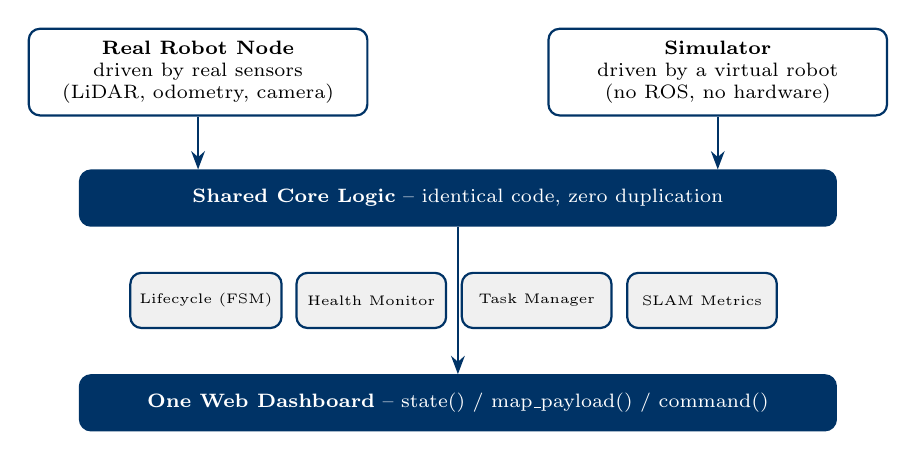
\begin{tikzpicture}[
      box/.style={rectangle,rounded corners,draw=uniblue,thick,minimum width=4.3cm,minimum height=1.1cm,align=center,font=\scriptsize},
      corebox/.style={rectangle,rounded corners,draw=uniblue,fill=uniblue,text=white,thick,minimum width=9.6cm,minimum height=0.7cm,align=center,font=\scriptsize},
      sub/.style={rectangle,rounded corners,draw=uniblue,fill=lightgray,minimum width=1.9cm,minimum height=0.7cm,align=center,font=\tiny},
      >=Stealth,thick
    ]
    \node[box] (real) at (0,3.6) {\textbf{Real Robot Node}\\driven by real sensors\\(LiDAR, odometry, camera)};
    \node[box] (sim) at (6.6,3.6) {\textbf{Simulator}\\driven by a virtual robot\\(no ROS, no hardware)};

    \node[corebox] (core) at (3.3,2.0) {\textbf{Shared Core Logic} -- identical code, zero duplication};

    \node[sub] (fsm) at (0.1,0.7) {Lifecycle (FSM)};
    \node[sub] (health) at (2.2,0.7) {Health Monitor};
    \node[sub] (task) at (4.3,0.7) {Task Manager};
    \node[sub] (slam) at (6.4,0.7) {SLAM Metrics};

    \node[corebox] (dash) at (3.3,-0.6) {\textbf{One Web Dashboard} -- state() / map\_payload() / command()};

    \draw[->,uniblue] (real.south) -- ++(0,-0.35) -| (core.north -| real);
    \draw[->,uniblue] (sim.south) -- ++(0,-0.35) -| (core.north -| sim);
    \draw[->,uniblue] (core) -- (dash);
  \end{tikzpicture}
  \end{center}
  {\tiny Both backends expose the exact same 3 functions, so the dashboard can't tell -- and doesn't need to know -- whether it's watching a real Tortugabot or a simulated one.}
\end{frame}

% --- 7: How the Virtual World Is Built ---
\begin{frame}{How the Virtual World Is Built}
  \footnotesize
  Four pieces of physics stand in for the real robot's sensors and drivers.
  \begin{columns}[T]
    \begin{column}{0.24\textwidth}
      \begin{block}{Map Source}
        \tiny Loads a real, previously-saved map if one exists. If none exists, it generates a synthetic maze arena instead.
      \end{block}
    \end{column}
    \begin{column}{0.24\textwidth}
      \begin{block}{Virtual Sensing}
        \tiny A ``reveal radius'' around the simulated robot uncovers the map gradually as it moves.
      \end{block}
    \end{column}
    \begin{column}{0.24\textwidth}
      \begin{block}{Path Planning}
        \tiny Its own A* search with obstacle inflation -- a self-contained stand-in for the real navigation planner.
      \end{block}
    \end{column}
    \begin{column}{0.24\textwidth}
      \begin{block}{Virtual Target}
        \tiny A red cube that wanders the map, so the follow-cube task can be tested without a camera.
      \end{block}
    \end{column}
  \end{columns}
  \vspace{0.3cm}
  \begin{block}{Runs standalone}
    \footnotesize
    A background thread ticks the virtual world 10 times a second -- the same update rate the real robot uses -- using only Python's standard library. No ROS, no GPU, no extra installs: it runs on any laptop.
  \end{block}
\end{frame}

% --- 8: Fault Injection ---
\begin{frame}{Fault Injection -- Breaking the Robot on Purpose}
  \footnotesize
  The one test a real robot can never safely run: deliberately killing a sensor mid-mission to prove recovery works.
  \begin{columns}[T]
    \begin{column}{0.52\textwidth}
      \begin{enumerate}
        \footnotesize
        \item Operator flips a toggle on the dashboard (e.g. ``kill LiDAR'')
        \item That component's heartbeat is silently withheld -- nothing else in the code path is touched or faked
        \item Health Monitor ages it past WARN, then DOWN -- the exact same logic used for a real failure
        \item Lifecycle is driven into FAULT for real -- zero velocity, task cancelled, state forced
        \item Toggle released $\rightarrow$ heartbeat resumes $\rightarrow$ full recovery, back to INITIALIZING, re-verified from scratch
      \end{enumerate}
    \end{column}
    \begin{column}{0.44\textwidth}
      \begin{block}{Why this proves something real}
        \footnotesize
        Nothing about the FAULT state itself is faked. Only the sensor's heartbeat is withheld -- the Health Monitor, the FSM, and the recovery path are the real production code, discovering a real missing signal.

        \vspace{0.15cm}
        On the physical robot, testing this would mean unplugging a live sensor while it drives. In simulation it's one click, fully repeatable, and safe to run as many times as needed.
      \end{block}
    \end{column}
  \end{columns}
\end{frame}

% --- 9: Simulator vs. Real Dashboard ---
\begin{frame}{Simulator vs.\ Real Dashboard}
  \small
  Same product experience, different world underneath -- and new abilities the real robot doesn't have.
  \vspace{0.2cm}
  \begin{columns}[T]
    \begin{column}{0.48\textwidth}
      \begin{block}{Identical in both}
        \footnotesize
        \begin{itemize}
          \item \textcolor{green!70!black}{The web dashboard UI, unchanged}
          \item \textcolor{green!70!black}{State machine and its transition rules}
          \item \textcolor{green!70!black}{Health thresholds and OK/WARN/DOWN logic}
          \item \textcolor{green!70!black}{``One task at a time'' task rules}
          \item \textcolor{green!70!black}{Navigation goal tolerance \& timeout values}
        \end{itemize}
      \end{block}
    \end{column}
    \begin{column}{0.48\textwidth}
      \begin{block}{Different in simulation}
        \footnotesize
        \begin{itemize}
          \item \textcolor{red!90!black}{Data comes from virtual physics, not real sensors}
          \item \textcolor{red!90!black}{Faults can be deliberately triggered on demand}
          \item \textcolor{red!90!black}{No lab access or physical robot required at all}
          \item \textcolor{red!90!black}{Runs anywhere -- stdlib only, zero setup}
          \item \textcolor{red!90!black}{Generates its own map when none exists yet}
        \end{itemize}
      \end{block}
    \end{column}
  \end{columns}
  \vspace{0.05cm}
  {\footnotesize \textbf{Why it matters:} the whole mission logic can be demoed, tested, and hardened for rare or risky scenarios -- safely, repeatably, and without ever touching the physical robot.}
\end{frame}

% --- 10: Simulation Dashboard (final slide of this section) ---
\begin{frame}{Simulation Dashboard}
  \begin{figure}
    \centering
    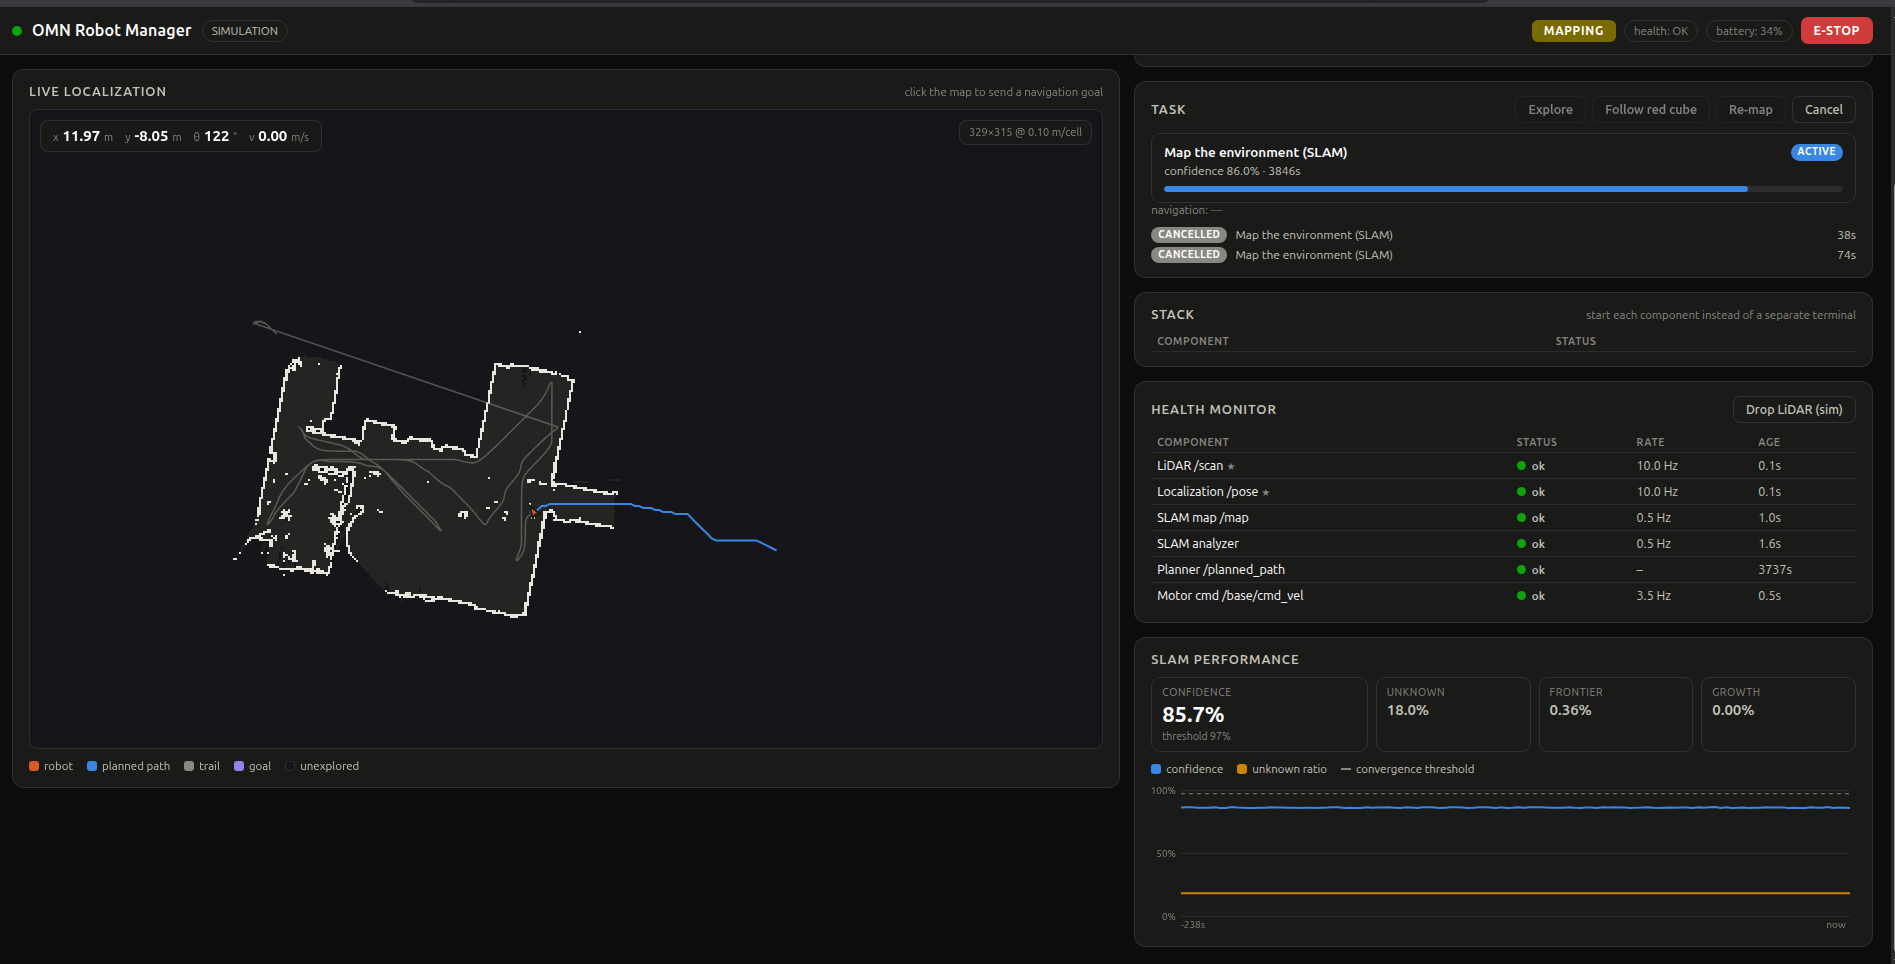
\includegraphics[width=0.88\linewidth]{img/robot_manager/simulation_dashboard.png}
  \end{figure}
\end{frame}







% ============================================================================
% NAVIGATION (Parts: Stuck, Smoothing, theta* vs a*)
% ============================================================================
\presentationsection[Navigation (stuck, smoothing, theta* v a*)]{Navigation (stuck, smoothing, theta* v a*)}
%\section{Path Smoothing}
\begin{frame}{Path Smoothing via LOS}
  \begin{columns}[T]
    \begin{column}{0.48\textwidth}
      \begin{block}{LOS-Algorithm}
        \small
        \begin{itemize}
          \item Path from A* gets checked for shortcuts
          \item Line of Sight is used
          \item Starts from first point, checks for 50 cells ahead
          \item Looks at furthest away, moves closer until visible
          \item Repeat for the next point
        \end{itemize}
      \end{block}
    \end{column}
    
    \begin{column}{0.48\textwidth}
      \begin{block}{Reasons for/against using}
        \small
        \begin{itemize}
          \item \textcolor{green!70!black}{For:} Very smooth path
          \item \textcolor{green!70!black}{For:} Decreased number of waypoints
          \item \textcolor{green!70!black}{For:} Changeable Look-Ahead-Distance
          \item \textcolor{red!90!black}{Against:} High computational Cost
          \item \textcolor{red!90!black}{Against:} Too slow for constant path replanning
          \item Result: Not used
        \end{itemize}
      \end{block}
    \end{column}
  \end{columns}



\end{frame}
\begin{frame}{Path Smoothing via Gradient}
  \begin{columns}[T]
    \begin{column}{0.48\textwidth}
      \begin{block}{Algorithm}
        \small
        \begin{itemize}
          \item Path from A* gets corrected
          \item Multiple passes
          \item Each coordinate gets tied to its origin
          \item Gets pulled away by: y\_next + y\_prev - 2.0 * y\_curr
          \item Stops automatically after specified passes or little change occurring
        \end{itemize}
      \end{block}
    \end{column}
    
    \begin{column}{0.48\textwidth}
      \begin{block}{Reasons for/against using}
      \small
        \begin{itemize}
          \item \textcolor{green!70!black}{For:} Low Computational Cost
          \item \textcolor{green!70!black}{For:} Tweakable
          \item \textcolor{red!90!black}{Against:} Path not as smooth
          \item \textcolor{red!90!black}{Against:} Might drag path through walls
          \item Result: Used
        \end{itemize}
      \end{block}
    \end{column}
  \end{columns}
\end{frame}


\begin{frame}{Theta*}
  \large
  Essentially A* with shortcuts:
  \begin{itemize}
    \item Performs shortcut checks to find shorter path
    \item Checks the current parent for visibility of best neighbor
    \item If successful, skips current node and uses parent as parent of best neighbor
    \item Repeat
  \end{itemize}
\end{frame}

%\section{Theta* vs A*}
\begin{frame}{Theta* vs A*}
  \vspace{-0.5cm}
  \begin{columns}[T]
    \begin{column}{0.5\textwidth}
      \begin{center}
        Theta*\\
        \vspace{0.2cm}
        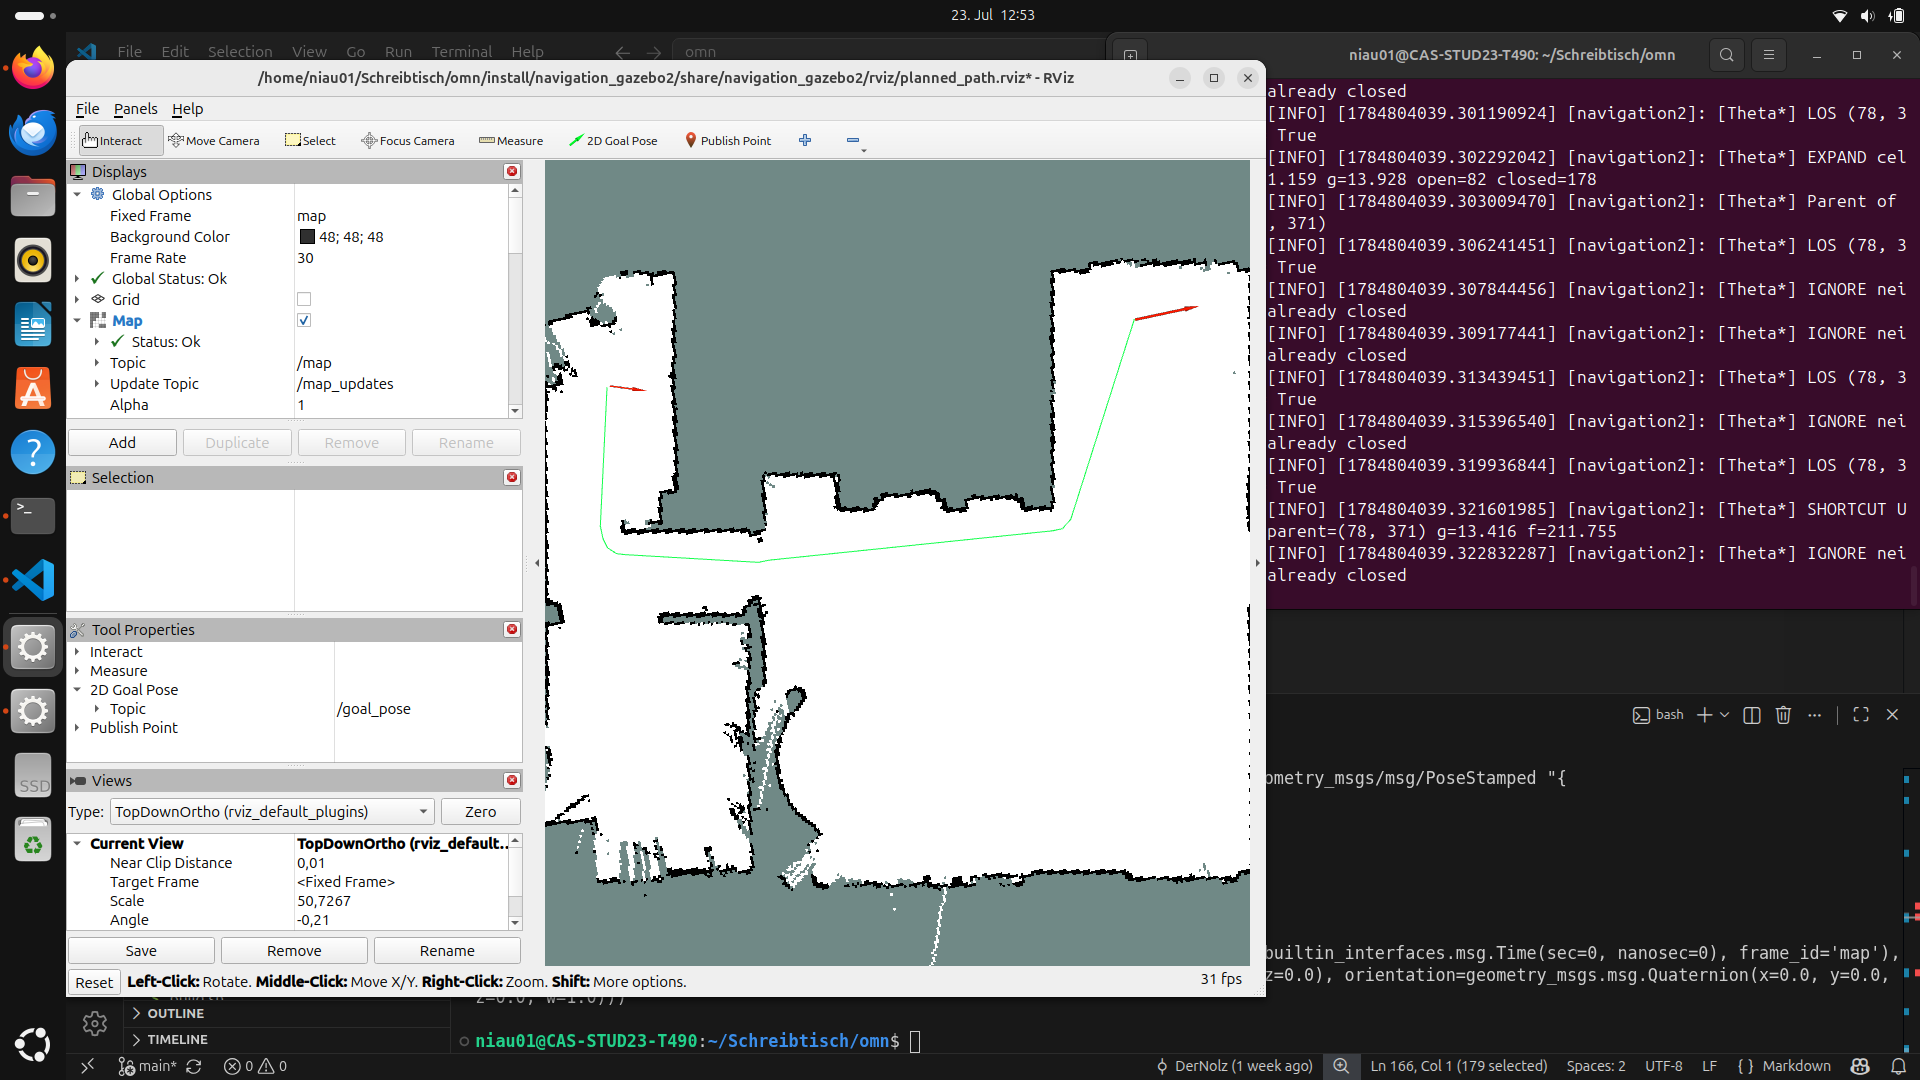
\includegraphics[width=\textwidth,height=0.65\textheight,keepaspectratio]{img/Theta_Path.png}
        Time of Computation: approx. 240 Seconds
        Noticeably smoother path
      \end{center}
    \end{column}
    
    \begin{column}{0.5\textwidth}
      \begin{center}
        A*\\
        \vspace{0.2cm}
        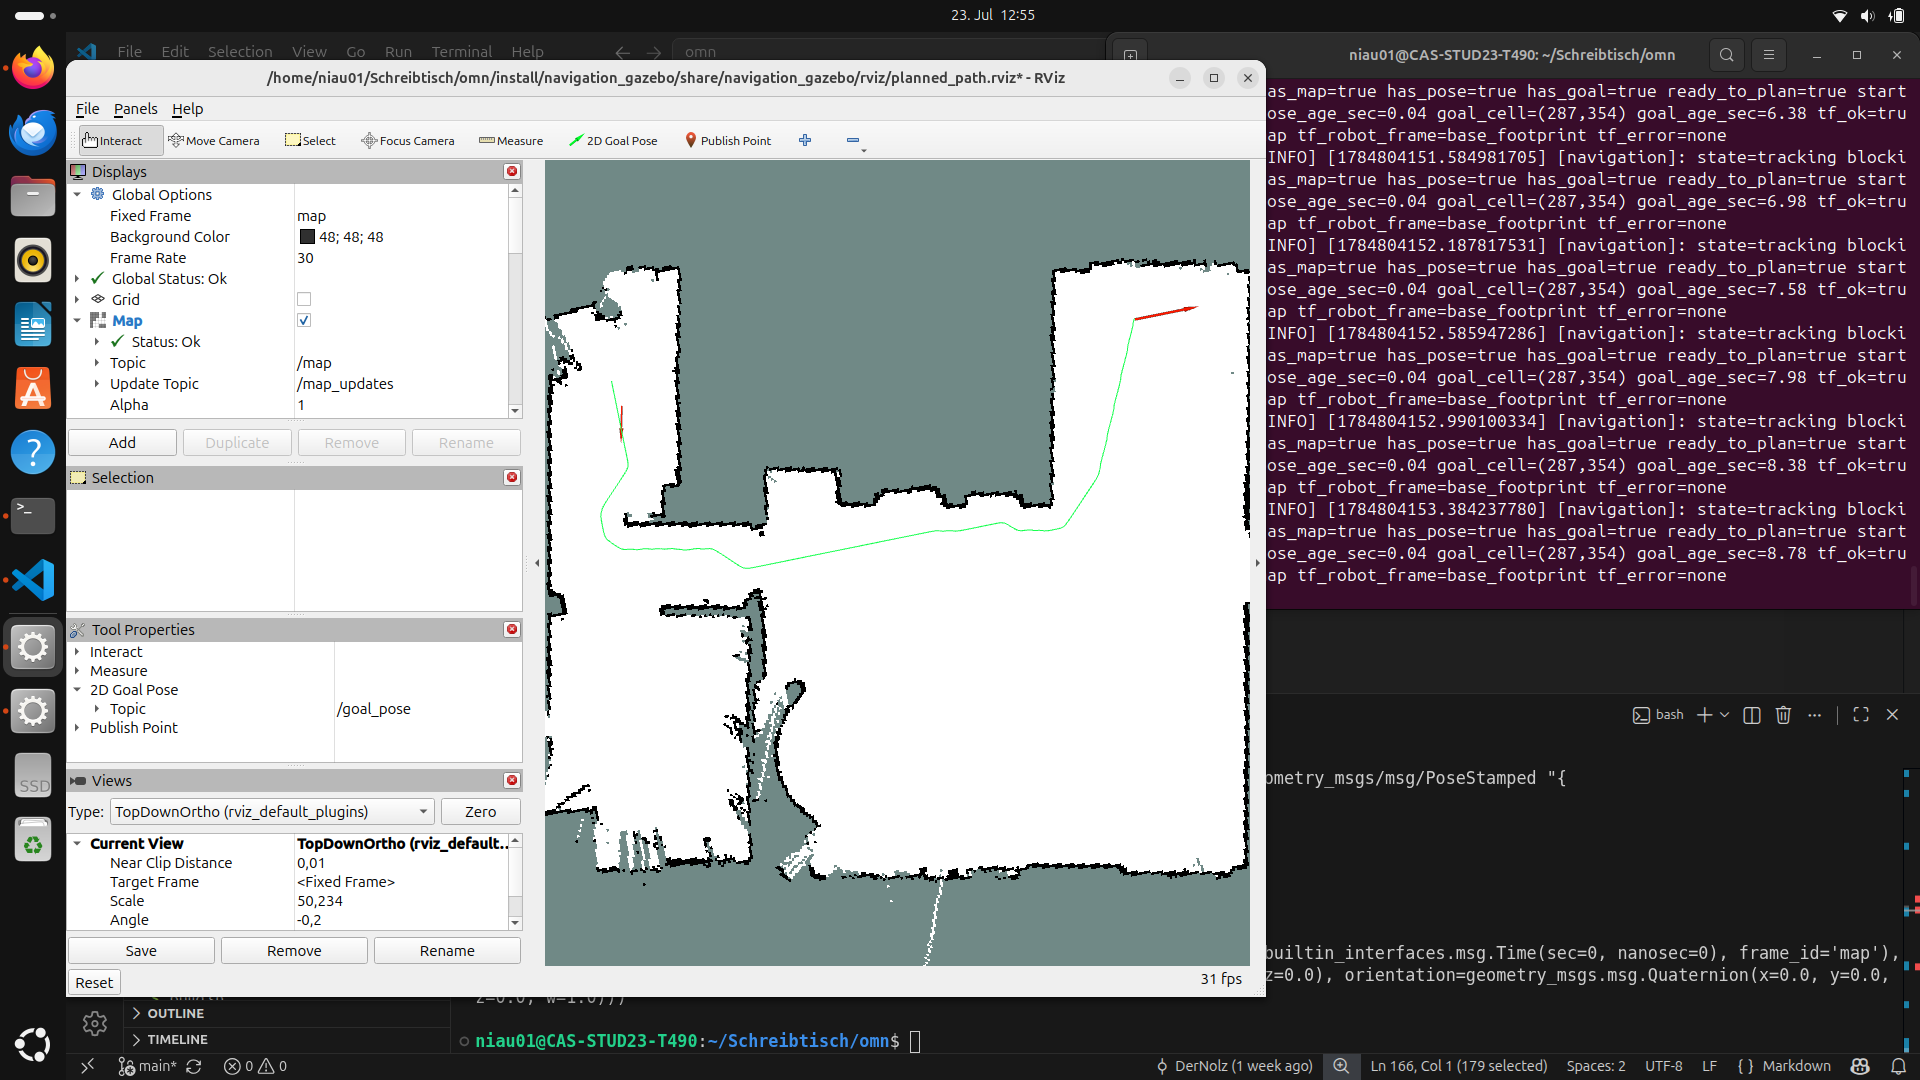
\includegraphics[width=\textwidth,height=0.65\textheight,keepaspectratio]{img/A_Path.png}
        Time of Computation: approx. 2 seconds
        Rougher path even after path smoothing
      \end{center}
    \end{column}
  \end{columns}
  \begin{center}
    \vspace{0.3cm}
    ==> A* used due to faster computation
  \end{center}
\end{frame}


%\section{Stuck Logic}
\begin{frame}{Stuck Logic}
  \vspace{-0.2cm}
  \begin{block}{Algorithm}
    \small
    \begin{itemize}
      \setlength\itemsep{-0.2em}
      \item Only when in mode "tracking" to avoid timeout while calculating path
      \item Checks weather the robot has moved enough in a specified timeframe
      \item When stuck, clears the current path and publishes velocities = 0
      \item When next\_goal in queue, switch over
    \end{itemize}
  \end{block}
  \vspace{-0.3cm}
  \begin{block}{Toggle Logic}
    \small
    \vspace{-0.3cm}
    \begin{columns}[T]
      \begin{column}{0.58\textwidth}
        \vspace{0.1cm}
        \hspace{2cm}
        Set toggle to false, when:
        \vspace{-0.2cm}
        \begin{itemize}
          \setlength\itemsep{-0.3em}
          \item goal is reached or new current goal detected
          \item stuck and there is a next goal
          \item path is cleared, there is no path or a new path was created
          \item not ready to plan (no pose, no map or no goal)
          \item replanning
        \end{itemize}
      \end{column}
      \begin{column}{0.38\textwidth}
        \vspace{0.1cm}
        Set toggle to true, when:
        \vspace{-0.2cm}
        \begin{itemize}
          \item following a path
        \end{itemize}
      \end{column}
    \end{columns}
  \end{block}
\end{frame}

% ============================================================
% GOAL QUEUE LOGIC
% ============================================================

\begin{frame}[t]{Goal Queue: Problem and Solution}
\small

\begin{columns}[T,onlytextwidth]
\begin{column}{0.48\textwidth}
\begin{block}{Previous Behaviour}
\begin{itemize}
    \item Navigation handled only one goal
    \item New goal replaced the active goal
    \item Older goals were discarded
\end{itemize}
\end{block}
\end{column}

\begin{column}{0.48\textwidth}
\begin{block}{New Behaviour}
\begin{itemize}
    \item Added FIFO goal queue
    \item Current goal stays active
    \item New goals wait in queue
    \item Goals follow received order
\end{itemize}
\end{block}
\end{column}
\end{columns}

\vspace{0.25cm}

\begin{block}{FIFO Order}
\centering
\Large Goal A $\rightarrow$ Goal B $\rightarrow$ Goal C
\end{block}

\end{frame}


\begin{frame}[t,shrink=8]{Goal Queue: Main Logic}

\begin{columns}[T,onlytextwidth]

\begin{column}{0.55\textwidth}
\begin{block}{When a New Goal Arrives}
\begin{enumerate}
    \item Transform the goal into the map frame
    \item Check whether it is a duplicate
    \item Activate it if no goal is active
    \item Otherwise, append it to the queue
    \item Reject it if the queue is full
\end{enumerate}
\end{block}
\end{column}

\begin{column}{0.40\textwidth}
\begin{block}{Queue Settings}
\begin{itemize}
    \item Minimum spacing: 0.25 m
    \item Maximum size: 100 goals
    \item New goals added with:
\end{itemize}

\begin{center}
\texttt{append()}
\end{center}

\begin{itemize}
    \item Next goal taken with:
\end{itemize}

\begin{center}
\texttt{popleft()}
\end{center}
\end{block}
\end{column}

\end{columns}

\vspace{0.2cm}

\begin{block}{Code Added In}
\begin{itemize}
    \item Import section and \texttt{\_\_init\_\_()}
    \item \texttt{goal\_pose\_callback()}
    \item New \texttt{activate\_next\_goal()} method
    \item Goal-reached part of \texttt{timer\_callback()}
\end{itemize}
\end{block}

\end{frame}


\begin{frame}[t,shrink=6]{Goal Queue: Simulation Result}

\begin{columns}[T,onlytextwidth]

\begin{column}{0.49\textwidth}
\begin{block}{Waypoint Queued}
\centering
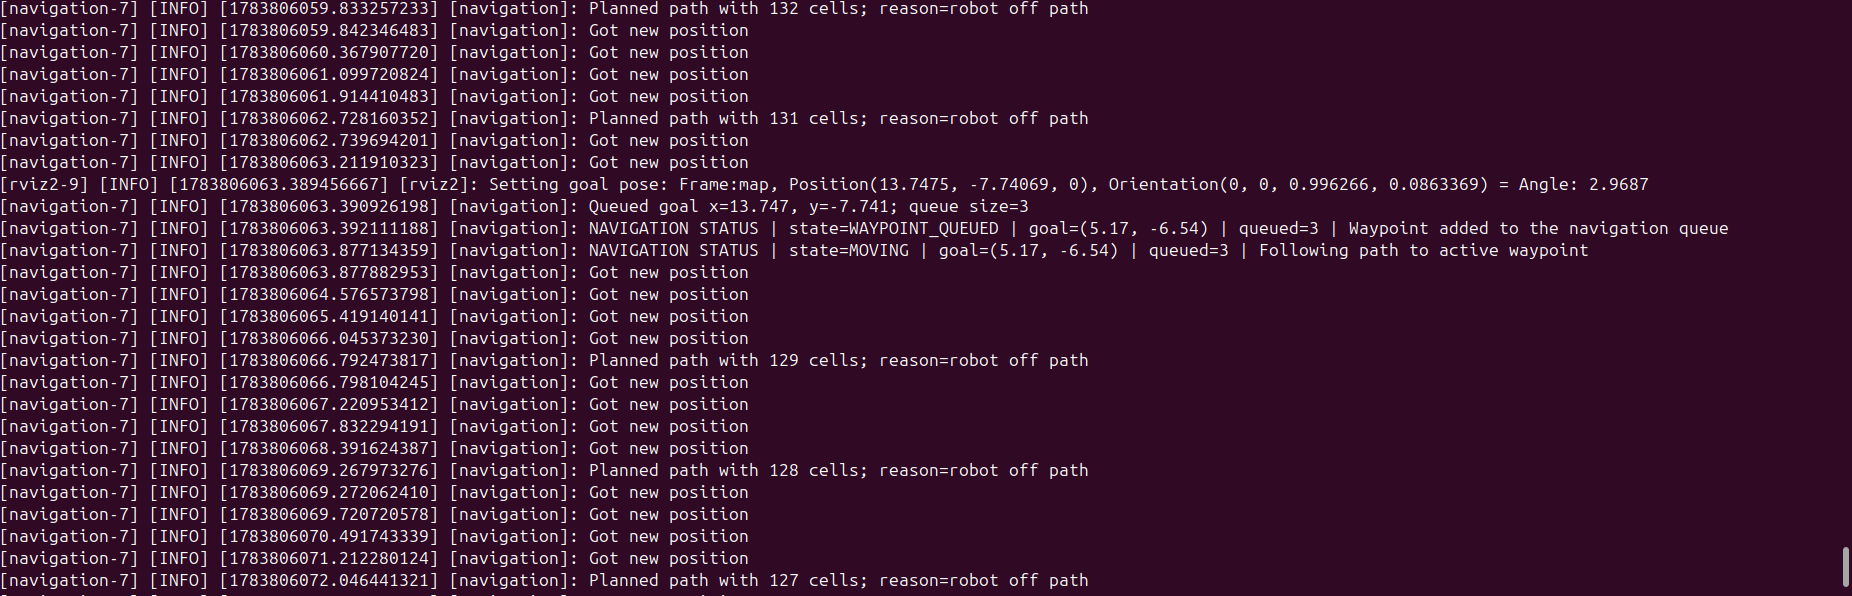
\includegraphics[width=\textwidth,height=0.35\textheight,keepaspectratio]{img/goal_queue_queued.png}

\begin{itemize}
    \item Queue size reached 3
    \item Active goal was not replaced
\end{itemize}
\end{block}
\end{column}

\begin{column}{0.49\textwidth}
\begin{block}{Queue Completed}
\centering
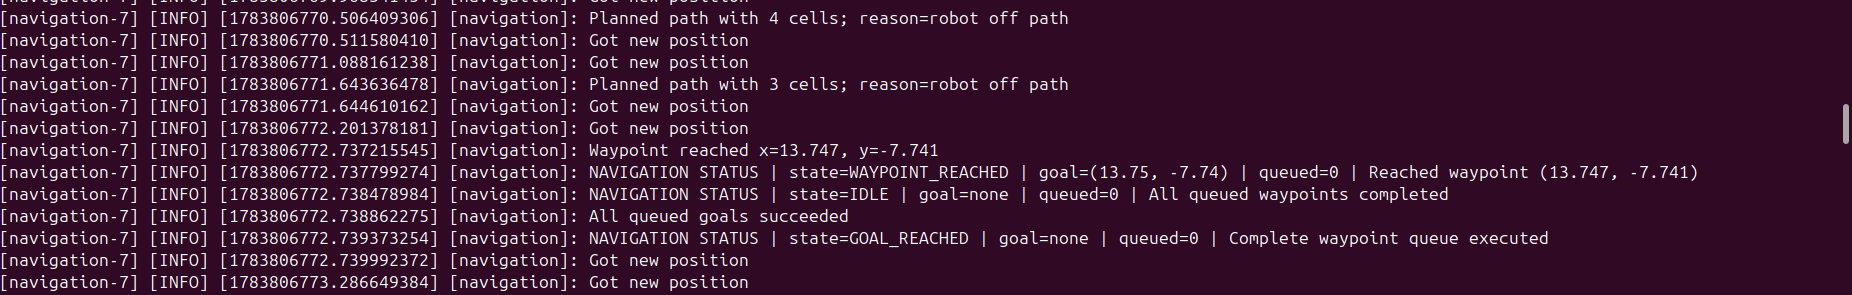
\includegraphics[width=\textwidth,height=0.35\textheight,keepaspectratio]{img/goal_queue_completed.png}

\begin{itemize}
    \item Queue returned to 0
    \item All queued goals succeeded
\end{itemize}
\end{block}
\end{column}

\end{columns}

\vspace{0.1cm}

\begin{block}{Result}
\centering
Goals are executed sequentially and are no longer discarded.
\end{block}

\end{frame}



% ============================================================================
% LOCALIZATION (IN SIM)
% ============================================================================
\presentationsection[Localization (in Sim)]{Localization (in Sim)}
\begin{frame}{Localization Prerequisites}
  \begin{columns}[T]
    \begin{column}{0.5\textwidth}
      \begin{block}{The robot knows:}
          \begin{itemize}
            \item Odometry (drifts)
            \item Map
            \item LaserScan (noisy)
          \end{itemize}
          But not its location
      \end{block}
    \end{column}
    
    \begin{column}{0.5\textwidth}
      \begin{block}{So we need:}
          \begin{itemize}
            \item Initial Pose
            \item Next Pose based on Odom
            \item Correct based on LiDAR-Data and Map
          \end{itemize}
      \end{block}
    \end{column}
  \end{columns}
\end{frame}


\begin{frame}{Localization Logic}
  \begin{columns}[T]
    \begin{column}{0.5\textwidth}
      \begin{block}{Basic Logic}
          \begin{itemize}
            \item Initial Pose is given
            \item Odom is added to Pose (Covariance grows)
            \item LaserScan gets matched to map (Covariance declines)\\
                (Search window only in proximity allowed)
            \item Pose set to LaserScan pose
          \end{itemize}
      \end{block}
    \end{column}
    
    \begin{column}{0.5\textwidth}
      \begin{block}{Deeper Logic}
          \begin{itemize}
            \item Covariance grows more with more movement
            \item Once Covariance grows too much, global search is started
            \item Global search is set the the new pose
          \end{itemize}
      \end{block}
    \end{column}
  \end{columns}
\end{frame}


\begin{frame}{LaserScan Matcher Logic}
  \begin{columns}[T]
    \begin{column}{0.5\textwidth}
      \begin{block}{Basic Logic}
          \begin{itemize}
            \item LaserScan converted to 2D coordinates in map
            \item Score assigned to poses in search window based on likelihood field
            \item Best score becomes new pose
          \end{itemize}
      \end{block}
    \end{column}
    
    \begin{column}{0.5\textwidth}
      \begin{block}{Deeper Logic}
          \begin{itemize}
            \item Three search stages (coarse, medium, fine)
            \item Each stage gets narrower/smaller
            \item Score assigned to poses based on:
              \begin{itemize}
                  \item closeness to odom estimation
                  \item closeness to the likelihood field (gaussian distribution)
              \end{itemize}
          \end{itemize}
      \end{block}
    \end{column}
  \end{columns}
\end{frame}


\begin{frame}{Global Search Logic}
  \begin{columns}[T]
    \begin{column}{0.5\textwidth}
      \begin{block}{Basic Logic}
          \begin{itemize}
            \item Takes many random poses in map and scores them
            \item Best matched score gets set to new pose
            \item Covariances get set low again
          \end{itemize}
      \end{block}
    \end{column}
    
    \begin{column}{0.5\textwidth}
      \begin{block}{Problems}
          \begin{itemize}
            \item Score Logic gets drawn to walls
            \item Problem with global search
            \item Closest spot to walls always wins
          \end{itemize}
      \end{block}
    \end{column}
  \end{columns}
  \begin{block}{Result}
    Fails almost everytime \\
    Reason that initial pose has to be given
  \end{block}
\end{frame}


\begin{frame}{Localization Performance}
  \begin{columns}[T]
    \begin{column}{0.5\textwidth}
      \begin{block}{Performance with initial pose}
          \begin{itemize}
            \item Tracks consistently
            \item Sometimes problems with hard turns
          \end{itemize}
      \end{block}
    \end{column}
    
    \begin{column}{0.5\textwidth}
      \begin{block}{Performance with global search}
          \begin{itemize}
            \item First pose almost always wrong
            \item Does not recover due to proximity scoring
          \end{itemize}
      \end{block}
    \end{column}
  \end{columns}
  \begin{block}{Possible Fixes and Future Work}
    \begin{itemize}
        \item Switch to particle tracking
        \item Tweak scoring
        \item Increase covariance more with turns
    \end{itemize}
  \end{block}
\end{frame}










% ============================================================================
% ============================================================================
% ============================================================================
% ============================================================================
% ============================================================================
% ============================================================================
% ============================================================================
% ============================================================================
% ============================================================================
% ============================================================================
% ============================================================================
% ============================================================================
% ============================================================================
% ============================================================================
% ============================================================================
% ============================================================================
% ============================================================================
% ============================================================================
% ============================================================================
% ============================================================================
% ============================================================================
% EVERYTHING BELOW THIS IS "COMMENTED OUT": IT WILL NOT BE DISPLAYED
\iffalse
% (if you want to remove this, also remove the "\if" later in the document)

% ============================================================================
\presentationsection[Requirements Identified]{Requirements Identified}
% ============================================================================

\begin{frame}{Requirements Identified}
  \begin{itemize}
    \item Metrics to quantify localization and navigation performance (For anomaly detection)
    \item Anomaly detection (Single source and Multiple source)
    \item Feature vectors for Anomaly Prediction
    \item Anomaly Prediction FOL Rule Derivation
    \item Scenario based and log based predictions
    \item Implement as Python script (*.py) or package that includes the complete pipeline
  \end{itemize}
\end{frame}

% ============================================================================
\presentationsection[Data Overview and Pre-processing]{Data Overview and Pre-processing}
% ============================================================================

\begin{frame}{Dataset Overview}
  \begin{columns}[T]
    \begin{column}{0.48\textwidth}
      \begin{block}{Dataset Properties}
        \begin{itemize}
          \item \textbf{Total Scenarios:} 100 directories
          \item \textbf{Runs per Scenario:} 3 (labeled 0, 1, 2)
          \item \textbf{Total Runs:} $\sim$300 experiments
          \item \textbf{Robot:} TurtleBot4 (0.22m diameter)
        \end{itemize}
      \end{block}
      
      \vspace{0.3cm}
      
      \begin{block}{Environment Types}
        \begin{itemize}
          \item door-width
          \item door-size
          \item room-size
          \item hallway-window
        \end{itemize}
      \end{block}
    \end{column}
    
    \begin{column}{0.48\textwidth}
      \begin{block}{File Structure per Run}
        \footnotesize
        \begin{tabular}{@{}l l@{}}
          \toprule
          \textbf{File} & \textbf{Content} \\
          \midrule
          poses.csv & Robot trajectories \\
          behaviors.csv & BT execution logs \\
          rosbag2.csv & ROS2 bag + AMCL \\
          scenario.config & Goals, params \\
          run.yaml & Run metadata \\
          \bottomrule
        \end{tabular}
      \end{block}
    \end{column}
  \end{columns}
\end{frame}

\begin{frame}{Pre-processing Steps}
  \begin{itemize}
    \item \textbf{Data Synchronization}: Aligns the robot's estimated position with the ``Ground Truth'' (actual capabilities) data.
    \vspace{0.2cm}
    \item \textbf{Stationary Filtering}: Removes irrelevant data where the robot was not moving, typically at the start or end of a run.
    \vspace{0.2cm}
    \item \textbf{Coordinate \& Orientation Normalization}:
    \vspace{0.2cm}
    \item \textbf{Yaw Normalization}: Normalizes all yaw angles to the range $[-\pi, \pi]$.
    \vspace{0.2cm}
    \item \textbf{Quaternion Conversion}: Converts orientation data from quaternion $(w,x,y,z)$ to yaw angles for easier error calculation.
  \end{itemize}
\end{frame}

% ============================================================================
\presentationsection[Performance Metrics and Features]{Performance Metrics and Features}
% ============================================================================

\begin{frame}{Performance Metrics (8 Metrics)}
  \begin{table}
    \footnotesize
    \renewcommand{\arraystretch}{1.2}
    \begin{tabular}{@{}L{3.8cm} c L{4.5cm} L{2.2cm}@{}}
      \toprule
      \textbf{Metric} & \textbf{Unit} & \textbf{Description} & \textbf{Category} \\
      \midrule
      mean\_pos\_error & m & Average position error & Localization \\
      rmse\_pos & m & Root mean square error (spike sensitive) & Localization \\
      mean\_yaw\_error & rad & Average orientation error & Localization \\
      executed\_path\_length & m & Total path traveled & Path \\
      path\_efficiency & ratio & gt\_path / executed (1 is best) & Path \\
      mean\_linear\_velocity & m/s & Average movement speed & Kinematics \\
      trajectory\_smoothness & rad/s² & Angular acceleration (lower = smoother) & Kinematics \\
      duration & s & Total run time & Kinematics \\
      mean\_amcl\_uncertainty & m & Average localization confidence & AMCL \\
      \bottomrule
    \end{tabular}
  \end{table}
\end{frame}

\begin{frame}{Features for Causal Analysis (27 Features)}
  \begin{table}
    \tiny
    \renewcommand{\arraystretch}{1.3}
    \begin{tabular}{@{}L{2.0cm} L{6.0cm} L{4.5cm}@{}}
      \toprule
      \textbf{Anomaly Type} & \textbf{Primary Predictors} & \textbf{Secondary Predictors} \\
      \midrule
      \textbf{Collision} & near\_wall, tight\_clearance, near\_static\_obstacle, clearance\_ratio & min\_wall\_distance, min\_obstacle\_distance \\
      \textbf{Stuck} & in\_narrow\_corridor, in\_small\_room, tight\_obstacle\_clearance & corridor\_width, room\_area \\
      \textbf{Goal Failure} & goal\_near\_wall, waypoint\_in\_tight\_space, door\_too\_narrow & goal\_wall\_distance, door\_width \\
      \textbf{Localization Uncertainty} & high\_noise, noise\_level & --- \\
      \textbf{Path Inefficiency} & obstacle\_clearance\_ratio, num\_obstacles, total\_obstacle\_area & min\_door\_narrow, goal\_through\_door \\
      \bottomrule
    \end{tabular}
  \end{table}
\end{frame}

% ============================================================================
\presentationsection[Anomaly Detection and Classification]{Anomaly Detection and Classification}
% ============================================================================

\begin{frame}{Anomaly Detection and Classification}
  \begin{columns}[T]
    \begin{column}{0.5\textwidth}
      \textbf{Rule-Based Anomalies (8 Types)}
      
      \vspace{0.2cm}
      
      \footnotesize
      \begin{itemize}
        \item \textbf{goal\_failure}: Goal not reached
        \item \textbf{no\_initiation}: Robot didn't start
        \item \textbf{position\_error\_spike}: Sudden errors
        \item \textbf{stuck}: Robot stopped moving
        \item \textbf{high\_amcl\_uncertainty}: Poor localization
        \item \textbf{high\_yaw\_error}: Orientation issues
        \item \textbf{path\_inefficiency}: Sub-optimal path
        \item \textbf{oscillation}: Jerky motion (smoothness $>$ 2.0)
      \end{itemize}
    \end{column}
    
    \begin{column}{0.45\textwidth}
      \textbf{ML-Based Anomaly Detection}
      
      \vspace{0.2cm}
      
      \small
      \textbf{Isolation Forest} trained on 8 standardized metrics:
      \begin{itemize}
        \item Captures multi-metric abnormal patterns missed by rules
        \item Unsupervised learning for outlier detection
      \end{itemize}
    \end{column}
  \end{columns}
\end{frame}

\begin{frame}{Anomaly Detection Results}
  \begin{columns}[T]
    \begin{column}{0.55\textwidth}
      \begin{center}
        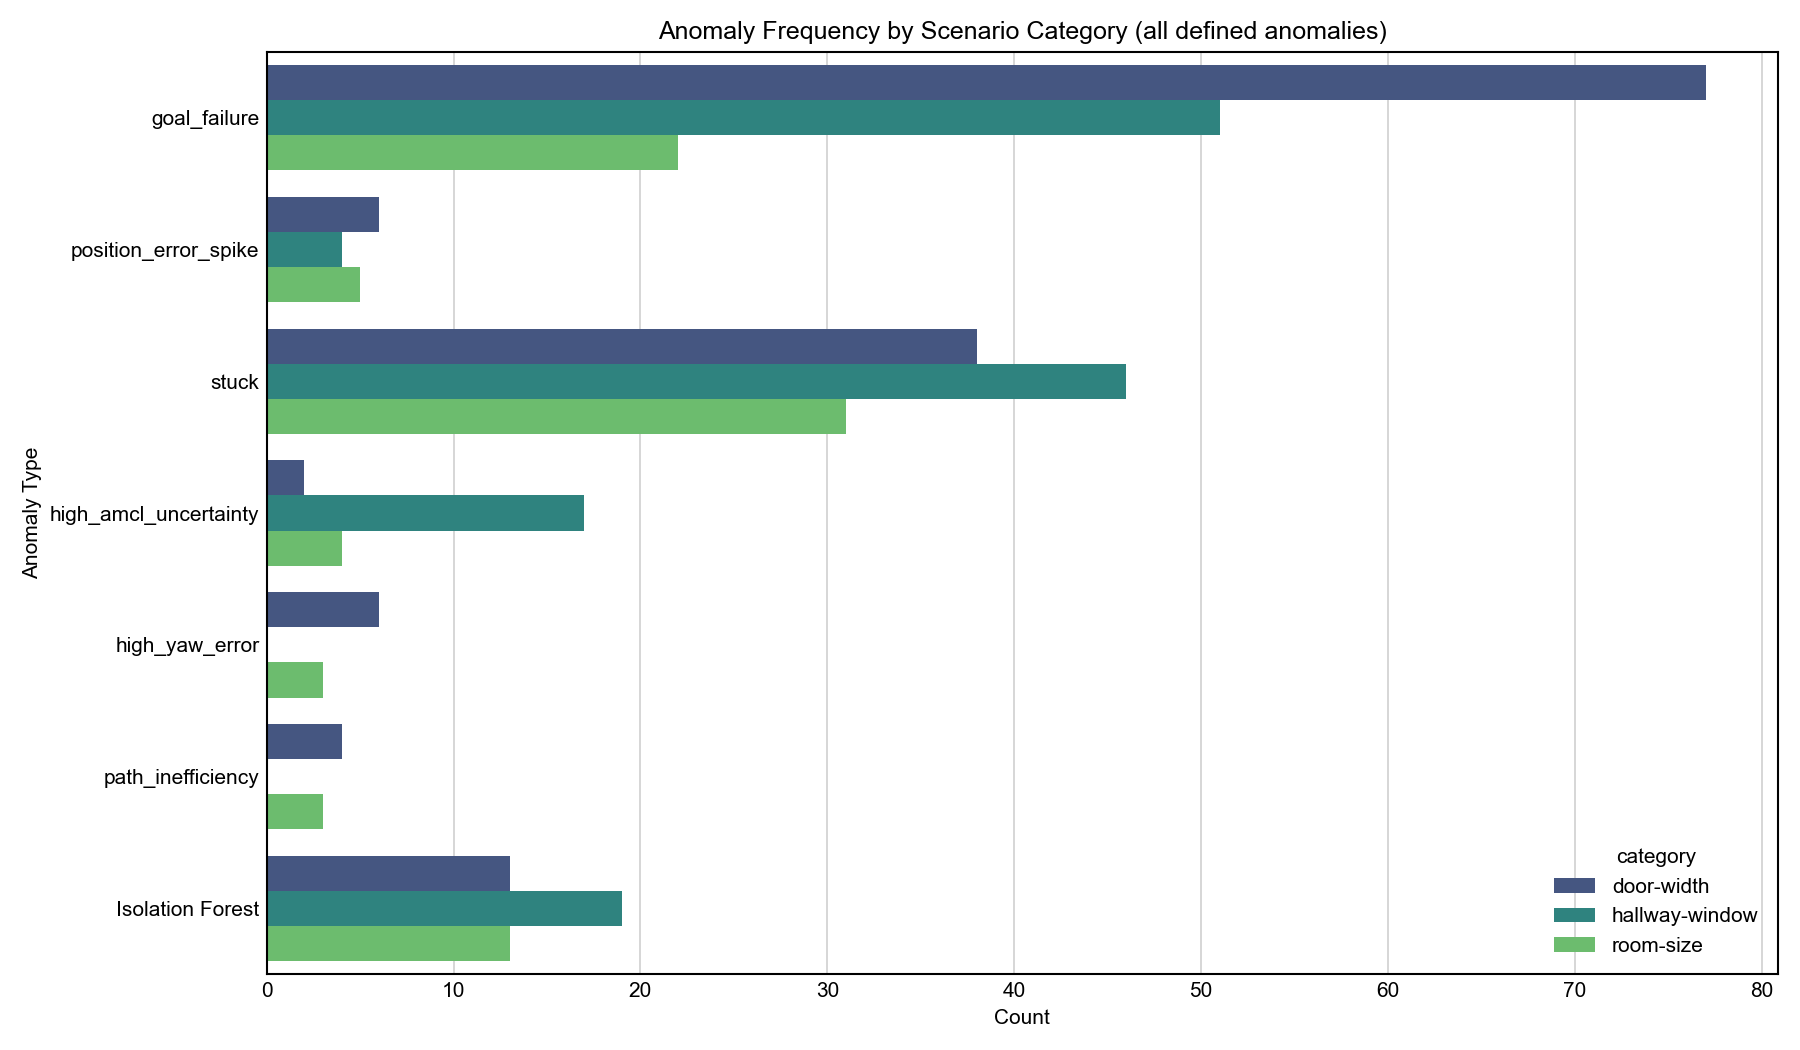
\includegraphics[width=\textwidth,height=0.65\textheight,keepaspectratio]{img/anomaly_by_category.png}
      \end{center}
    \end{column}
    
    \begin{column}{0.42\textwidth}
      \textbf{Key Findings}
      
      \vspace{0.3cm}
      
      \begin{itemize}
        \item Total occurrences: \textbf{341}
        \item \textcolor{accentred}{\textbf{goal\_failure}} is most common (50\%)
        \item \textbf{stuck} follows at 38.3\%
        \item \textbf{Isolation Forest} catches 15\%
        \item Single run can have multiple anomalies
      \end{itemize}
    \end{column}
  \end{columns}
\end{frame}

% ============================================================================
% ============================================================================
\presentationsection[Correlations Analysis]{Correlations Analysis}
% ============================================================================

\begin{frame}{Anomaly Correlations Analysis}
  \begin{itemize}
    \item \textbf{position\_error\_spike + high\_yaw\_error} (Jaccard = 0.60)
    \begin{itemize}
      \item[$\rightarrow$] Poor orientation tracking leads to position drift
    \end{itemize}
    
    \vspace{0.5cm}
    
    \item \textbf{high\_yaw\_error + path\_inefficiency} (Jaccard = 0.78)
    \begin{itemize}
      \item[$\rightarrow$] Orientation errors cause inefficient path execution
    \end{itemize}
  \end{itemize}
\end{frame}

% ============================================================================
\presentationsection[Early Prediction Insights]{Early Prediction Insights}
% ============================================================================

\begin{frame}{Early Prediction: Predictability}
  \begin{table}
    \small
    \renewcommand{\arraystretch}{1.3}
    \begin{tabular}{@{}L{3.5cm} C{2.0cm} C{2.0cm} C{1.5cm}@{}}
      \toprule
      \textbf{Anomaly} & \textbf{PR-AUC} & \textbf{ROC-AUC} & \textbf{Cases} \\
      \midrule
      goal\_failure & 0.852 & 0.828 & 150 \\
      stuck & 0.766 & 0.789 & 115 \\
      Isolation Forest & 0.661 & 0.834 & 45 \\
      \bottomrule
    \end{tabular}
  \end{table}
\end{frame}

\begin{frame}{Early Multi-features and Anomaly Correlation}
  \begin{columns}[T]
    \begin{column}{0.32\textwidth}
      \begin{block}{\textbf{Stuck}}
        \footnotesize
        \begin{itemize}
          \item path\_length: r=-0.491 
          \item std\_velocity: r=-0.437 
          \item path\_efficiency: r=-0.384 
        \end{itemize}
      \end{block}
    \end{column}
    
    \begin{column}{0.32\textwidth}
      \begin{block}{\textbf{Goal Failure}}
        \footnotesize
        \begin{itemize}
          \item duration: r=+0.524 
          \item mean\_angular\_vel: r=-0.283 
          \item path\_length: r=+0.276 
        \end{itemize}
      \end{block}
    \end{column}
    
    \begin{column}{0.32\textwidth}
      \begin{block}{\textbf{high\_amcl\_uncertainty}}
        \footnotesize
        \begin{itemize}
          \item rmse\_pos: r=+0.291 
          \item max\_velocity: r=+0.277 
          \item std\_pos\_error: r=+0.274 
        \end{itemize}
      \end{block}
    \end{column}
  \end{columns}
\end{frame}

% ============================================================================
\presentationsection[Causality Analysis Methodology]{Causality Analysis Methodology}
% ============================================================================

\begin{frame}{Methodology Evolution}
  \begin{center}
    \textbf{Simple Decision Tree} $\rightarrow$ \textbf{Ensemble Model} $\rightarrow$ \textbf{Surrogate Model}
    
    \vspace{0.5cm}
    
    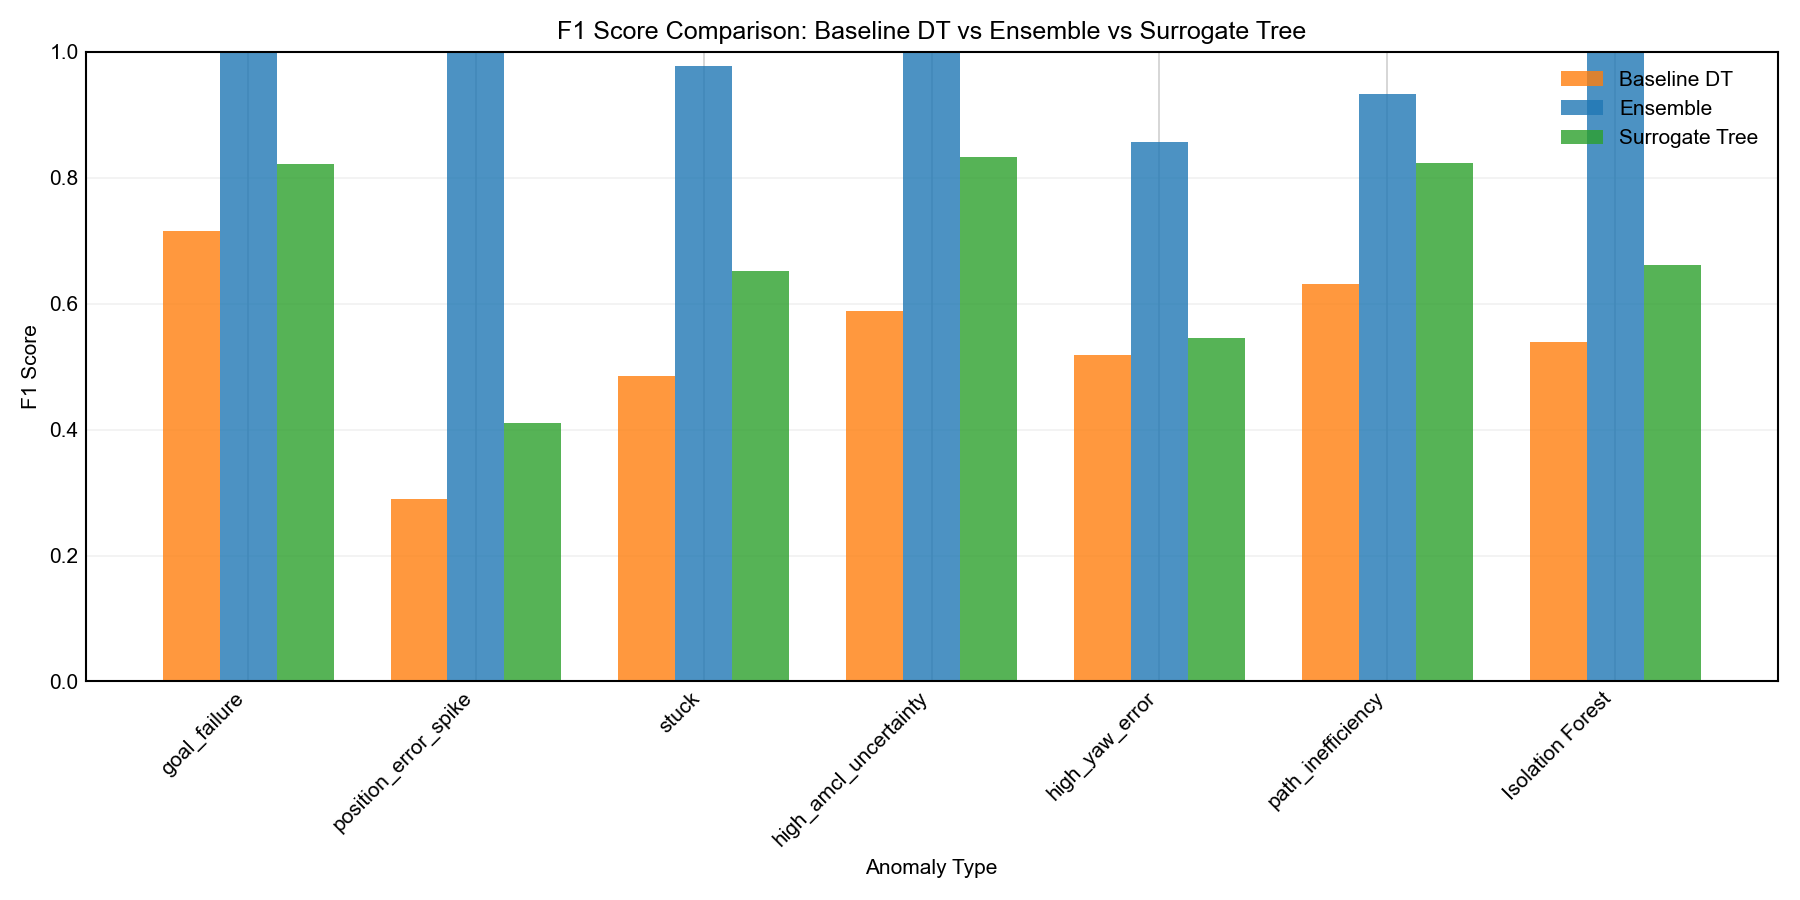
\includegraphics[width=0.85\textwidth,height=0.6\textheight,keepaspectratio]{img/model_comparison_f1.png}
  \end{center}
\end{frame}

\begin{frame}{Current Approach}
  \begin{itemize}
    \item \textbf{Step 1: High-Capacity Model Training (Ensemble)}
    \begin{itemize}
      \item[$\rightarrow$] Voting Classifier: Decision Tree + Random Forest + Gradient Boosting
      \item[$\rightarrow$] Separate trees for both log-based and scenario-based predictions
      \item[$\rightarrow$] Prioritizes F1-score
    \end{itemize}
    
    \vspace{0.2cm}
    
    \item \textbf{Step 2: Surrogate Model Training (Distilled Decision Tree)}
    \begin{itemize}
      \item[$\rightarrow$] Separate trees for both log-based and scenario-based predictions
      \item[$\rightarrow$] Constrained tree (max\_depth=4)
      \item[$\rightarrow$] Target: Ensemble predictions (not ground truth)
    \end{itemize}
    
    \vspace{0.2cm}
    
    \item \textbf{Step 3: Rule Extraction}
    \begin{itemize}
      \item[$\rightarrow$] Extract paths with P(Anomaly) $>$ 0.5
    \end{itemize}
    
    \vspace{0.2cm}
    
    \item \textbf{Step 4: FOL Translation}
    \begin{itemize}
      \item[$\rightarrow$] Map thresholds to semantic predicates
    \end{itemize}
  \end{itemize}
\end{frame}

\begin{frame}{What is a Decision Tree / Surrogate Model?}
  \begin{center}
    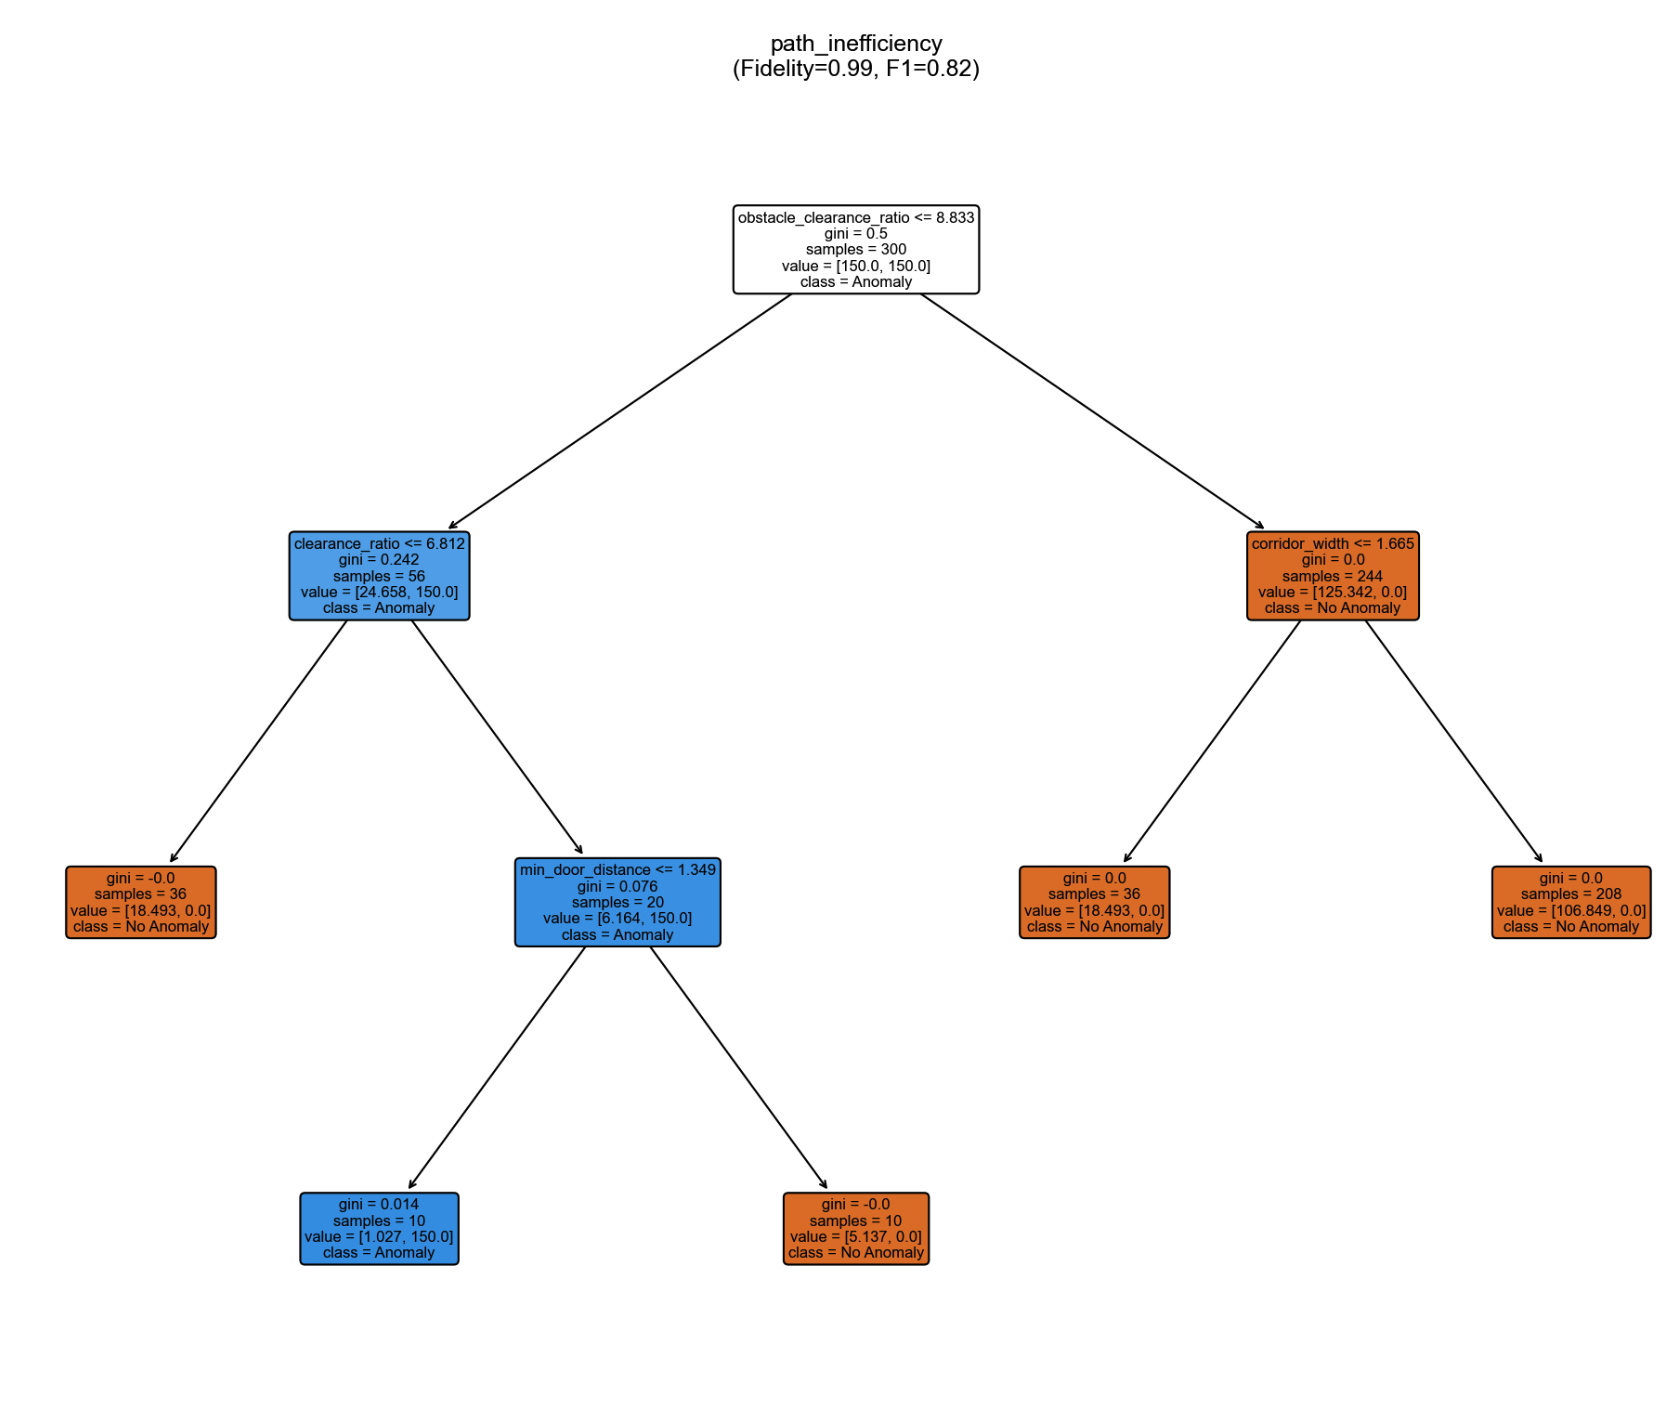
\includegraphics[width=0.9\textwidth,height=0.6\textheight,keepaspectratio]{img/DT.png}
  \end{center}
  
  \vspace{0.3cm}
  
  \footnotesize
  \textbf{Why Surrogate?} Captures ensemble's knowledge in an interpretable tree structure, enabling FOL rule extraction while maintaining high fidelity ($>$90\%).
\end{frame}

% ============================================================================
\presentationsection[Insights]{Insights}
% ============================================================================

\begin{frame}{Technical Insights (Important)}
  \begin{enumerate}
    \item \textbf{Better quality rules with just scenario information}
    \begin{itemize}
      \item In case of many anomalies it showed better predictive power and generalization (F1 score and other metrics) when just used scenario description, robot information, and environment JSON file for deriving FOL rules instead of also including more informative logs, CSV files.
    \end{itemize}
    
    \vspace{0.4cm}
    
    \item \textbf{Surrogate Distillation}
    \begin{itemize}
      \item Ensemble models achieve higher accuracy, but surrogate trees provide 90\%+ fidelity with full interpretability.
      \item Surrogate trees were even simpler than simple decision trees yet showed better results (F1, confusion metrics).
    \end{itemize}
  \end{enumerate}
\end{frame}

\begin{frame}{Domain and Methodological Insights}
  \begin{enumerate}
    \item \textbf{Narrow Door Width is Critical}: Doors $<$ 1.8× robot footprint cause $>$60\% of goal failures
    
    \vspace{0.2cm}
    
    \item \textbf{Sensor Noise Cascades}: High noise ($>$0.05) correlates with both localization errors AND path inefficiency
    
    \vspace{0.2cm}
    
    \item \textbf{Corridor Navigation is Challenging}: Narrow corridors ($<$3× footprint) are disproportionately associated with stuck states
    
    \vspace{0.2cm}
    
    \item \textbf{Static Obstacles Compound Difficulty}: Scenarios with obstacles + narrow passages have 2× failure rate
    
    \vspace{0.2cm}
    
    \item \textbf{Generalization Requires Feature Abstraction}: Relative features (clearance ratios) generalize better than absolute measurement numbers
  \end{enumerate}
\end{frame}

% ============================================================================
\presentationsection[Summary]{Summary}
% ============================================================================

\begin{frame}{Summary}
  \begin{center}
    \Large\textcolor{uniblue}{\textbf{Team 4 Final Presentation}}\\
    \vspace{0.5cm}
    \normalsize Thank you!\\
    \vspace{0.3cm}
    Questions?
  \end{center}
\end{frame}
\fi
% END CONTENT IMPORTED FROM omn.tex

\end{document}
